%---------------------------------------------------------------------------%
%-                          国科大开题报告 LaTeX 工程                         -%
%-                   基于 ucasproposal 模板 (mohuangrui/ucasproposal)         -%
%---------------------------------------------------------------------------%
%->> Document class declaration
%---------------------------------------------------------------------------%
\documentclass{Style/ucasproposal}%
%- 可选参数:
%- [<oneside|twoside|print>]% 单面打印/双面打印/纸质打印
%- [fontset=<adobe|none|...>]% 指定字体集，默认自动检测
%- [scheme=plain]% 留学生英文模式
%---------------------------------------------------------------------------%
%->> Document settings
%---------------------------------------------------------------------------%
\usepackage[bibtex,numbers,xhf,tikz]{Style/artratex}% 数字引用[1]+无页眉页脚
%- [bibtex|biber]% 参考文献处理引擎
%- [numbers|super|authoryear|alpha]% 引用样式，numbers=数字上标式
%- [xhf]% 关闭页眉页脚
%- [list]% 代码与算法列表环境
%- [tikz]% TikZ 绘图
\usepackage{Style/artracom}% 用户自定义命令
%-
%->> 用户自定义设置（请在下方添加，勿修改模板文件）
%---------------------------------------------------------------------------%
\usepackage{booktabs}% 三线表（自因变量表、基准计划表等）
\usepackage{etoolbox}% 章节命令补丁
\pretocmd{\section}{\clearpage}{}{}% 每个大章另起一页
\usetikzlibrary{arrows.meta,fit,backgrounds}% 技术路线图所需 TikZ 库
%- TikZ 样式定义（技术路线图源节点样式）
\tikzset{
  module/.style={draw, rounded corners=2pt, align=left, text width=13cm, inner sep=6pt, font=\small},
  smallbox/.style={draw, rounded corners=2pt, align=center, inner sep=6pt, font=\small},
  arr/.style={-{Stealth[length=2.5mm]}, thick},
  darr/.style={-{Stealth[length=2.5mm]}, thick, dashed},
  layerbox/.style={draw, densely dashed, inner sep=8pt},
  layerlabel/.style={font=\small\bfseries},
}
%---------------------------------------------------------------------------%
%->> Document inclusion
%---------------------------------------------------------------------------%
%\includeonly{Tex/01-background,Tex/02-related}% 选择性编译
%---------------------------------------------------------------------------%
%->> Document content
%---------------------------------------------------------------------------%
%-
%-> 封面信息
%-
%---------------------------------------------------------------------------%
%->> 封面信息（请填写个人信息）
%---------------------------------------------------------------------------%
%-
%-> 中文封面信息
%-
\schoollogo{scale=0.112}{ucas_logo}% 校徽
\title{基于智能体的漏洞挖掘与修复技术研究}% 报告题目
\author{（待填）}% 作者姓名
\authorid{2025xxxxxxxx}% 学号（待填）
\advisor{XXX}% 指导老师（待填）
\advisortitle{研究员}% 指导老师职称（待填）
\degree{博士}% 学位：硕士、博士
\degreetype{工学}% 学位类别：理学、工学、工程、医学等
\major{网络空间安全}% 二级学科专业名称
\field{漏洞挖掘与修复}% 研究方向
\institute{中国科学院信息工程研究所}% 院所
\chinesedate{2026~年~09~月}% 日期
%---------------------------------------------------------------------------%
%
\begin{document}
%-
%-> 前置部分：封面、目录
%-
\pagenumbering{roman}% 罗马页码
\input{Tex/Frontmatter}% 封面 + 目录
%-
%-> 主体部分
%-
\clearpage
\pagenumbering{arabic}% 阿拉伯页码
%---------------------------------------------------------------------------%
%->> 正文章节
%---------------------------------------------------------------------------%
\section{选题的背景及意义}
\label{sec:background-significance}

\subsection{选题背景}
\label{sec:research-background}

安全漏洞是系统中可被威胁源利用或触发、导致安全策略被违反的缺陷或弱点，可能损害信息的保密性、完整性或系统的可用性\cite{nist_vulnerability}。本课题主要关注软件与固件实现中的漏洞。与一般功能缺陷相比，漏洞分析不仅需要识别异常行为，还需要确定其触发条件与安全影响，程序是否崩溃并不是判断漏洞存在的唯一依据。

漏洞治理并不止于发现缺陷或发布补丁，而是涉及漏洞发现与报告、复现确认与根因分析、影响评估与优先级划分、修复或缓解措施制定、补丁验证、协调披露与发布，以及部署后的修复状态核查等环节\cite{cert_cvd_2017,sokavr,fiber}。这些环节连接漏洞发现者、软件开发者与部署维护者，既要回答漏洞在哪里、如何修复，也要确认修复是否有效、是否体现在实际运行的程序中。因此，单个环节的自动化并不能替代对后续修复结果的确认。

近年来，大语言模型的代码理解与生成能力，为漏洞治理提供了新的技术途径。通过结合代码检索、调试、编译和测试工具，智能体能够根据执行反馈调整分析过程，逐步完成漏洞调查与程序修改。Big Sleep 已展示在真实开源软件中发现未知漏洞的能力，PatchAgent 则将缺陷定位、补丁生成与验证整合到交互式修复流程中\cite{bigsleep,patchagent}。这些进展为降低漏洞分析和修复对人工操作的依赖提供了基础，也使研究重点进一步转向复杂任务条件下的分析深度与结果可靠性。

在漏洞挖掘方面，源码可用、执行环境完备且错误判据明确时的分析能力，不能直接等同于受限场景下的发现能力。对于仅能获取设备或剥离符号二进制的嵌入式场景，程序语义恢复、内部状态观察与执行环境构建均受到限制\cite{binrex,fuzzware}。协议状态违例、行为逻辑错误和资源泄漏等问题又可能不立即产生崩溃，需要结合协议、接口及资源生命周期要求判断行为是否错误，因而不能仅依靠增加测试输入或代码覆盖解决\cite{oracleproblem}。

在漏洞修复方面，异常表现位置与实际需要修改的位置可能分属不同函数，局部代码和告警信息不足以完整解释漏洞根因\cite{li2024interpvd}。上下文缺失、根因理解偏差及边界条件遗漏，也可能使模型生成局部合理但修复不充分的补丁\cite{nong2025appatch}。在修复验证方面，通过已有测试并不意味着补丁在未覆盖的输入和执行路径上仍然正确\cite{smith2015cure}；上游补丁已经发布，也不能直接证明目标二进制包含对应修复\cite{fiber}。因此，补丁生成能力的提升还需要独立的修复有效性检查与目标产物修复状态核验相配合。

基于上述背景，本课题以“基于智能体的漏洞挖掘与修复技术研究”为题，围绕“发现问题—生成修复—确认修复”的主线，开展\textbf{基于智能体的漏洞挖掘、基于智能体的漏洞自动修复、基于智能体的漏洞修复验证}三个方向的研究，分别面向受限场景中的漏洞发现、根因驱动的补丁生成，以及修复有效性与目标产物修复状态的确认，提升漏洞治理关键环节的自动化水平与可靠性。

\subsection{选题意义}
\label{sec:research-significance}

在研究层面，本课题围绕安全要求与程序行为之间的对应关系，探索大模型语义推理与程序分析、动态测试相结合的方法。通过研究行为约束如何支持漏洞判定、根因理解如何指导有效修改，以及何种程序证据能够支持修复结论，有助于深化对不完备信息条件下智能体安全分析能力及其边界的认识。同时，区分漏洞发现、修复有效性与目标修复状态的评价依据，可为相关方法的设计和比较提供更明确的标准。

在应用层面，本课题有望提高嵌入式设备与二进制组件中隐蔽安全缺陷的发现能力，降低复杂漏洞定位与补丁编写的人工成本。通过同时关注安全要求与合法行为，减少不完整修复和功能回归；通过核查目标产物中的修复实现，帮助维护者识别补丁发布与实际修复状态之间的差异。相关成果可为软件安全维护、嵌入式设备审计和第三方组件更新核查提供技术支撑。

% \section{选题的背景及意义}

% \subsection{选题背景}

% \subsubsection{漏洞攻防格局正在发生深刻变化}

% 随着软件规模持续增长与软件供应链日益复杂，安全漏洞的数量、影响面与利用速度都在快速上升。一方面，国家级漏洞库中公开漏洞数量逐年攀升，攻击者利用公开漏洞信息实施"N-day 快速武器化"的窗口期不断缩短；另一方面，大量部署中的二进制组件缺乏透明、可验证的补丁状态，使下游用户与监管方难以判断"这个漏洞到底有没有被修复"。以 Log4j（CVE-2021-44228）为代表的事件表明：单一组件缺陷可以引发整个生态的修复验证难题~\cite{log4j}。

% 与此同时，以大语言模型（LLM）为核心的\textbf{智能体（Agent）}技术正以前所未有的速度进入软件安全领域。与传统"静态规则 + 人工操作"的分析模式不同，智能体通过"模型推理 + 工具调用 + 迭代反馈"的闭环，能够自主完成代码阅读、二进制分析、测试用例生成、补丁合成等过去高度依赖专家经验的任务。Google Project Zero 与 DeepMind 的 Big Sleep 项目首次展示了 AI 智能体在真实开源项目中发现未知内存安全漏洞的能力~\cite{bigsleep}；DARPA AIxCC 大赛则系统验证了智能体在"自动发现—自动修补—自动验证"全链路中的可行性~\cite{aixcc}。\textbf{智能体正从"辅助工具"演变为漏洞攻防闭环中的核心行动者}。

% \subsubsection{漏洞攻防闭环中的三个关键环节}

% 一个完整的漏洞攻防闭环，可以抽象为三个相互衔接的核心环节：

% \begin{enumerate}
%   \item \textbf{漏洞挖掘（Discovery）}：在目标软件中发现未知漏洞，回答"哪里可能有洞"。
%   \item \textbf{漏洞修复（Automated Vulnerability Repair, AVR）}：针对已确认存在的漏洞，自动定位并合成补丁，回答"怎么把洞补上"。
%   \item \textbf{漏洞修复验证（Repair Verification）}：判定修复是否真正消除漏洞根因、目标程序是否实际包含修复，回答"洞补上了没有、补得对不对"。
% \end{enumerate}

% 这三个环节覆盖了漏洞从"未知 $\rightarrow$ 已知 $\rightarrow$ 修复"的完整生命周期，彼此共享大量基础能力：对漏洞语义的理解、对补丁意图的建模、对二进制与源码之间语义鸿沟的桥接、对修复正确性的判定。\textbf{然而，现有研究大多将三者割裂对待}，分别由不同团队、不同工具链、不同基准独立推进，导致漏洞语义、补丁语义、修复语义在各自环节中被重复建模，既浪费资源，也阻碍了跨环节能力的复用。

% \subsubsection{智能体带来的新机遇与新问题}

% 智能体技术的引入，为统一上述三个环节提供了可能：

% \begin{itemize}
%   \item \textbf{能力侧}：前沿编码智能体已能熟练调用 binutils、Ghidra、gdb 等二进制与源码分析工具，完成多步推理与决策。
%   \item \textbf{成本侧}：token 成本与推理延迟的持续下降，使"在真实仓库级代码库上大规模运行智能体"从理想变为可行。
%   \item \textbf{生态侧}：SWE-bench~\cite{swebench}、CVE-Bench~\cite{cvebench}、AIxCC~\cite{aixcc} 等评测基准的成熟，为系统化比较不同智能体安全能力提供了基础设施。
% \end{itemize}

% 但与此同时，三个关键环节在智能体视角下仍各自存在未被充分回答的核心问题：

% \begin{itemize}
%   \item 在漏洞挖掘上，传统 fuzzing 与符号执行在语义/逻辑漏洞（如认证绕过、状态机错误、配置驱动缺陷）上进展缓慢，\textbf{核心难点是"自因变量"——那些不受外部输入控制、由内部状态/配置/时序决定的变量}——导致现有输入驱动方法在错误维度上爆炸。
%   \item 在漏洞修复上，智能体已能生成"看起来合理"的补丁，但\textbf{"补丁是否真正消除了漏洞根因"}这一判定问题（即 PPT 在修复场景下的对偶问题）仍缺乏可靠机制，导致现有基准上"补丁过拟合 PoC、回归失败、绕过检查"等问题频发~\cite{rrbench}。
%   \item 在漏洞修复验证上，智能体虽已展现出与专用系统相当甚至更优的补丁存在性测试（PPT）性能~\cite{zhang2026agenticppt}，但\textbf{补丁定位（patch localization）}仍是主要瓶颈，且\textbf{对"演化补丁"（patch evolution）的鲁棒性}尚未解决——这部分能力本质上是漏洞语义理解问题。
% \end{itemize}

% 由此可见，三个环节在智能体范式下并非彼此孤立，而是被一条隐含的主线紧密连接：\textbf{对漏洞—补丁—修复三者语义的统一建模与跨环节复用}。抓住这条主线，就有可能突破现有"单点智能体应用"的局限，构建面向完整攻防闭环的智能体安全分析体系。

% \subsubsection{选题的提出}

% 基于上述观察，本文提出"\textbf{基于智能体的漏洞挖掘与修复}"这一研究课题，以"漏洞语义—补丁语义—修复语义"的统一建模为核心，系统研究智能体在漏洞挖掘、漏洞自动修复、漏洞修复验证三个关键环节中的能力边界、瓶颈机理与增强方法，并探索三个环节之间的能力迁移与反馈闭环。

% \subsection{选题意义}

% \subsubsection{理论意义}

% \begin{enumerate}
%   \item \textbf{推动"智能体 + 程序分析"交叉范式的形成}：现有智能体安全研究多停留在"把 LLM 当作更强的分类器/生成器"层面，缺乏对智能体推理过程与程序分析约束之间关系的理论刻画。本课题将探索智能体的"观察—推理—行动"循环与污点分析、符号执行、规约验证等传统程序分析技术的耦合机制，为构建新型混合分析范式提供理论支撑。
%   \item \textbf{建立漏洞语义跨环节统一表示}：针对漏洞挖掘、修复、修复验证三环节语义割裂的现状，本课题尝试建立以"漏洞触发条件—补丁干预点—修复不变式"为核心的统一表示，为后续跨任务迁移学习、多任务智能体训练提供概念框架。
%   \item \textbf{深化对"自因变量"与"演化补丁"两类共性瓶颈的理解}：前者是漏洞挖掘的核心障碍，后者是 PPT 与修复共同面对的难点。本课题将从智能体视角对二者进行系统建模，形成可被后续研究复用的分析框架。
% \end{enumerate}

% \subsubsection{实践意义}

% \begin{enumerate}
%   \item \textbf{提升漏洞挖掘的自动化水平}：相比内存破坏漏洞，语义/逻辑漏洞（认证绕过、状态机错误、配置驱动缺陷）长期缺乏高效自动化检测手段。基于智能体的挖掘方法有望通过自然语言规约理解、内部状态推断与测试用例合成，显著扩展可检测漏洞类型。
%   \item \textbf{提高自动修复的可信度}：通过将 PPT 思想引入修复验证环节，本课题旨在构建"修复—验证"闭环，减少"补丁过拟合 PoC"、"修复引入回归"等问题，提升智能体生成补丁的真实可用率，为软件供应链的快速应急响应提供工具支撑。
%   \item \textbf{支撑大规模供应链安全审计与修复状态核查}：PPT 是软件物料清单（SBOM）与漏洞影响评估的关键技术，也是修复验证能力的直接应用。基于智能体的端到端 PPT 可显著降低对符号表与人工目标函数定位的依赖，提升对剥离二进制与真实发行版包的分析能力，对关键基础设施软件资产盘点与修复状态核查具有直接价值。
%   \item \textbf{服务国家网络空间安全战略}：漏洞攻防能力是国家网络空间安全的核心竞争力之一。本课题围绕智能体这一新兴技术形态，系统研究其在漏洞攻防关键环节中的应用边界与增强路径，可为我国在下一代自动化攻防体系建设中抢占先机提供理论与技术储备。
% \end{enumerate}
% 一、选题的背景及意义
\section{国内外本学科领域的发展现状与趋势}

本章围绕课题的三个研究点，分别梳理相关领域的研究背景、研究现状与趋势、以及尚存的关键挑战。其中，2.1 节对应语义漏洞挖掘研究点，2.2 节与 2.3 节分别对应拟开展的漏洞自动修复与漏洞修复验证研究。

\subsection{基于智能体的语义漏洞挖掘}

\subsubsection{研究背景}

漏洞挖掘旨在从目标软件中自动发现未知缺陷。经过数十年发展，以模糊测试（Fuzzing）、符号执行（Symbolic Execution）、污点分析（Taint Analysis）为代表的技术已在内存破坏类漏洞（缓冲区溢出、释放后使用等）上取得显著成功。然而，\textbf{在语义/逻辑漏洞（semantic / logic vulnerability）方面，自动化挖掘能力仍然薄弱}。

语义漏洞指程序在内存安全层面"合法"、但在设计意图或业务逻辑层面"错误"的缺陷，其典型类别包括：认证与授权绕过、状态机错误、配置驱动缺陷、第三方组件使用违规、跨组件逻辑错误等。与内存破坏漏洞不同，语义漏洞\textbf{不产生崩溃信号}，无法被 AddressSanitizer 等通用 oracle 直接捕获；其判定往往需要人工或半自动构造的策略/规约（policy/specification），这是语义漏洞挖掘区别于内存破坏挖掘的根本难点。

在 IoT 与嵌入式固件场景下，该问题尤为突出。固件通常包含大量由\textbf{内部状态、外设寄存器、NVRAM 配置、时序事件}共同决定的程序路径，这些路径对传统的输入驱动 fuzzing 而言几乎不可达。我们将这类"不受外部输入直接控制、由系统内部状态/配置/时序决定的变量"统称为\textbf{自因变量（Self-Caused Variables）}。自因变量普遍存在于认证逻辑、状态机转移、外设交互与配置处理中，是语义漏洞挖掘的核心障碍。

与此同时，大语言模型与智能体展现出前所未有的自然语言规约理解、跨抽象层推理与代码合成能力，为突破语义漏洞挖掘瓶颈提供了新的可能。智能体可以阅读协议 RFC、数据手册、配置说明等自然语言文档，自动提取安全不变量作为 oracle；可以在 fuzzing 循环中观察覆盖率停滞，主动推断需要翻转哪个内部状态变量，并合成对应的环境事件序列；还可以跨驱动层、RTOS 任务、应用层进行语义推理，识别跨层逻辑错误。

\subsubsection{研究现状与趋势}

\paragraph{（一）语义漏洞检测的传统方法}

围绕语义漏洞检测，已有研究沿多条技术路线展开：

\begin{itemize}
  \item \textbf{静态符号执行与模型检验}：Firmalice~\cite{firmalice} 以"认证绕过"为唯一语义，结合特权模型进行符号执行，是该方向的奠基性工作；FIE~\cite{fie} 面向 MSP430 固件进行全系统符号执行。此类方法受限于路径爆炸与环境建模难度，难以扩展到大型固件。
  \item \textbf{静态污点与数据流分析}：KARONTE~\cite{karonte} 通过跨二进制污点分析检测固件多进程通信中的逻辑缺陷；Operation Mango~\cite{operationmango}、FIRE~\cite{fire}、OctopusTaint~\cite{octopustaint}、UVScan~\cite{uvscan} 等工作进一步提升了可扩展性与检测精度；LATTE~\cite{latte} 首次将 LLM 引入二进制污点分析，显著降低了规则定制成本。
  \item \textbf{固件重托管与覆盖率 Fuzzing}：FIRM-AFL~\cite{firmafl}、P2IM~\cite{p2im}、Laelaps~\cite{laelaps}、Fuzzware~\cite{fuzzware}、Ember-IO~\cite{emberio} 等工作通过外设建模与精确 MMIO 处理，显著提升了固件 fuzzing 的覆盖率；Firmvenom~\cite{firmvenom} 引入外设语义感知 fuzzing，进一步提升效率。
  \item \textbf{状态感知 Fuzzing}：AFLNet~\cite{aflnet} 以协议状态机引导 fuzzing；StateAFL~\cite{stateafl} 通过内存快照推断协议状态；SyzTrust~\cite{syztrust} 面向可信执行环境，明确提出"隐藏状态变量缺乏语义反馈"这一与自因变量高度对应的概念，并通过状态感知 fuzzing 缓解深状态不可达问题。
  \item \textbf{配置驱动 Fuzzing}：CONFU~\cite{confu} 等工作将配置文件直接作为 fuzz 输入，绕开"配置变量在运行期不变"带来的自因性。
\end{itemize}

\paragraph{（二）自因变量的建模与求解}

针对自因变量带来的挑战，已有研究从不同角度提出了建模与求解思路，如表~\ref{tab:selfcaused} 所示。总体上，SOTA 已从不把自因变量当作噪声，而是将其\textbf{显式对象化}——或提升为 fuzzer 一等输入，或通过符号/学习方法恢复其生成模型。但\textbf{尚缺乏统一抽象来整合 state-driven / config-driven / timing-driven / peripheral-driven 等不同形态}。

\begin{table}[htbp]
  \centering
  \caption{自因变量建模的代表性方法路线}
  \label{tab:selfcaused}
  \small
  \begin{tabular}{p{3.4cm}p{4.2cm}p{6.6cm}}
    \toprule
    \textbf{方法路线} & \textbf{代表工作} & \textbf{核心思想} \\
    \midrule
    外设状态机学习 & P2IM, Laelaps, Fuzzware, Firmvenom & 将 MMIO 建模为状态机，符号执行 + 自动机学习推断状态转移 \\
    运行时状态推断 & StateAFL, SyzTrust & 内存快照聚类推断隐藏状态，将状态作为 fuzzer 一等公民 \\
    配置显式化 & CONFU & 将配置变量作为独立输入维度 \\
    反向数据流切片 & KARONTE, Operation Mango & 从 sink 反向切片，识别不受 source 控制的变量并单独求解 \\
    混合执行 & Laelaps, FirmHybridFuzz & 输入不可解时切换符号执行，将内部状态变量显式符号化 \\
    \bottomrule
  \end{tabular}
\end{table}

\paragraph{（三）智能体在漏洞挖掘中的初步探索}

2024 年以来，智能体在漏洞挖掘中的应用开始爆发：FirmAgent~\cite{firmagent} 将 fuzzing 与 LLM 智能体结合，由 fuzzing 提供污点源，LLM 智能体进行上下文感知分析与 PoC 生成，在 14 个真实固件上发现 182 个漏洞，精度 91\%，获得 17 个 CVE——这是目前该方向最强的公开结果；FirmPilot~\cite{firmpilot} 基于多智能体协作进行固件重托管，用 LLM 推断外设与环境语义；ChatAFL~\cite{chatafl} 利用 LLM 提取协议语法、丰富种子、突破覆盖率平台；Big Sleep~\cite{bigsleep} 首次公开展示 AI 智能体在真实开源项目中发现未知内存安全漏洞；AIxCC~\cite{aixcc} 系统验证了智能体在"发现—修补—验证"全链路中的能力。此外，BinReX~\cite{binrex} 提出的"语义检索 + 可验证推理"范式表明：为智能体提供检索增强的语义导航与机器可验证的证据链，相比单纯扩大模型规模或工具集更能提升二进制分析效果，这一范式对语义漏洞挖掘具有直接借鉴意义。

\paragraph{（四）研究趋势}

研究范式正从"LLM 作为分类器/生成器嵌入传统 pipeline"转向"智能体作为分析主体，自主规划分析路径"；研究对象从内存破坏漏洞扩展到语义/逻辑漏洞；系统架构从单智能体演进到规划—分析—验证分工的多智能体；评估对象从合成基准扩展到真实固件镜像与大型开源仓库。

\subsubsection{研究挑战}

\begin{enumerate}
  \item \textbf{自因变量缺乏统一形式化}：state-driven、config-driven、timing-driven、peripheral-driven 等不同形态的自因变量在文献中各自为战，缺乏类似污点分析中 lattice 的统一抽象，导致方法难以泛化。
  \item \textbf{语义 oracle 的自动构造}：逻辑漏洞的判定准则难以自动抽取，Firmalice 的认证绕过 oracle 使用十年仍是孤例。如何利用智能体从自然语言文档中自动提取安全不变量，是关键开放问题。
  \item \textbf{覆盖率反馈对语义深度的"失明"}：coverage-guided 机制对"已覆盖代码内的逻辑错误"无感知，需要语义感知的反馈信号来替代或增强传统边覆盖。
  \item \textbf{跨层语义鸿沟}：固件漏洞常跨越"驱动层 $\rightarrow$ RTOS 任务 $\rightarrow$ 应用层 $\rightarrow$ 云端/APP"，现有工具基本局限于单层，缺乏跨抽象层的语义整合能力。
  \item \textbf{基准缺失}：缺乏公认的"语义漏洞 + 自因变量"基准，导致不同方法之间难以公平比较。
\end{enumerate}

\subsection{基于智能体的漏洞自动修复}

\subsubsection{研究背景}

漏洞修复是软件安全维护的重要环节，其目标不仅是阻止已知攻击输入触发异常，还需要消除导致危险行为的程序缺陷，并维持正常使用所依赖的功能与安全约定。漏洞自动修复（Automated Vulnerability Repair，AVR）将漏洞分析、补丁生成与补丁验证组织为自动化过程，以降低安全维护对人工分析的依赖。与面向一般软件缺陷的自动程序修复（Automated Program Repair，APR）相比，AVR 更强调在攻击者可控输入、异常状态及安全敏感操作下恢复必要的安全条件。因此，修复目标不能仅用代码修改是否合理、程序能否编译或已知失败是否消失来描述，还应考察危险行为是否被有效约束，以及相关合法行为是否得到保留~\cite{sokavr}。

漏洞修复通常发生在不完备信息条件下。漏洞报告、检测器告警和概念验证程序（Proof of Concept，PoC）能够提供分析线索，但不一定直接指出应修改的程序位置，也不一定完整描述正确修复应满足的条件。已有 APR 研究表明，通过用于生成补丁的测试集，并不意味着补丁能够推广到未见输入~\cite{smith2015cure}。在漏洞修复中，这一问题进一步表现为：已知 PoC 不再触发，可能只是因为某个特定输入或执行分支被阻断，而非漏洞根因已经消除。由此，AVR 实际上包含两个相互关联、但不能相互替代的问题：\textbf{如何根据有限证据推断应当修复什么，以及如何验证生成的补丁确实满足修复要求}~\cite{sokavr,smith2015cure}。

大语言模型（Large Language Model，LLM）为处理漏洞描述、源代码和修复经验提供了新的技术途径。进一步结合代码检索、文件编辑、编译执行与测试工具，模型能够在智能体框架中逐步完成定位、修改和反馈驱动的修复。PatchAgent 等工作已经将这些环节整合到交互式系统中，推动研究对象从给定代码片段上的补丁生成扩展至真实项目中的自动修复~\cite{patchagent}。然而，交互能力的增强并不自动等同于修复语义的正确理解：系统仍需判断告警位置与根因位置之间的关系、识别跨函数依赖，并区分补丁通过当前验证与恢复完整安全要求之间的差别。

Rust 等系统编程语言使这一问题具有更丰富的语义层次。RustBelt 从形式化角度说明，基于 \texttt{unsafe} 实现的安全抽象需要满足相应验证条件，才能作为安全语言的可靠扩展~\cite{jung2018rustbelt}；针对真实 Rust 程序的研究也揭示了内存与线程安全实践中的复杂问题~\cite{qin2020rust}。因此，Rust 漏洞修复不仅涉及局部条件检查，还可能涉及所有权、生命周期、类型与 trait 约束、异常清理和并发状态。基于上述背景，本节围绕传统修复方法、LLM 与智能体修复、补丁正确性评价及 Rust 修复进展展开，重点讨论从漏洞表现恢复根因语义、从候选修改建立可信修复证据所面临的挑战。

\subsubsection{研究现状与趋势}

\paragraph{（一）基于搜索、程序合成与语义约束的传统修复}

传统 APR 为漏洞自动修复提供了候选搜索、修复位置选择和测试反馈等基础机制。Le Goues 等提出的 \textbf{GenProg} 通过遗传编程对程序进行变换，以失败测试与功能测试约束候选程序的选择~\cite{genprog}。Nguyen 等提出的 \textbf{SemFix} 将通过给定测试的要求编码为约束，并结合符号执行、约束求解和程序合成搜索修复表达式~\cite{nguyen2013semfix}。二者分别代表基于搜索和基于语义约束的修复思路，但主要面向一般程序缺陷，不能直接作为已覆盖多类安全漏洞的证据；其生成结果的可靠性还取决于所使用的测试、约束及允许的程序变换。

面向安全缺陷，研究进一步尝试从漏洞执行中提取比单次测试结果更强的修复条件。Gao 等提出的 \textbf{ExtractFix} 从崩溃或漏洞触发中提取约束，通过程序分析将其向候选修复位置传播，再合成满足约束的修改~\cite{gao2021extractfix}。该方法不只要求原始输入不再崩溃，而是将崩溃所违反的条件转化为修复义务，探索对输入变化更具一般性的修复。Zhang 等提出的 \textbf{VulnFix} 则利用程序状态快照、状态变异与归纳推断学习区分安全和危险状态的不变式，并据此生成补丁~\cite{zhang2022vulnfix}。这些研究说明，安全条件建模和反例反馈并非 LLM 出现后才引入的思想，传统语义方法已经为约束驱动修复提供了基础。

不过，这类方法的分析与合成建立在具体的漏洞模型、状态表示和候选修复空间之上。对于缺乏通用崩溃判据的权限、协议和状态逻辑问题，或者依赖复杂库语义的跨过程缺陷，单一崩溃约束难以完整表达修复要求；大型项目的路径、别名与环境建模也会增加分析成本~\cite{sokavr,gao2021extractfix,zhang2022vulnfix}。因此，传统方法的局限不宜简单归结为"缺乏语义分析"，而应理解为：已有语义表示与求解机制如何适应更复杂的安全要求，以及如何在精度与可扩展性之间取得平衡。

\paragraph{（二）从历史补丁学习到大语言模型生成}

学习式 AVR 将漏洞代码到修复代码的映射作为建模对象，从历史修复数据中获得候选生成能力。Fu 等提出的 \textbf{VulRepair} 基于 T5 类编码器—解码器架构，结合预训练与子词表示学习漏洞修复模式~\cite{fu2022vulrepair}。Zhou 等提出的 \textbf{VulMaster} 进一步扩展输入范围和信息来源，缓解代码截断及修复上下文不足的问题~\cite{zhou2024vulmaster}。这类方法降低了逐类手工设计补丁模板的需求，但仍需考虑训练数据覆盖、输入信息完整性以及评价方式的影响；与参考补丁相似，并不直接等同于恢复了相应安全性质。

随着通用代码模型的发展，研究开始探索不进行任务专门训练的修复方式。Pearce 等系统考察了\textbf{零样本漏洞修复}，通过组织漏洞代码与提示信息引导模型生成候选修改，展示了预训练模型迁移至安全修复任务的可能性~\cite{pearce2023zeroshot}。与面向固定数据分布的训练方式相比，提示式方法便于接入不同模型和额外上下文；但模型输出仍需接受程序级检查，提示中缺失的调用关系、错误处理约定或边界条件，不会因为模型具有代码生成能力而自动得到可靠补全。

训练式方法也在从修复结果拟合转向显式推理能力学习。Wen 等提出的 \textbf{Vul-R2} 结合领域推理数据、监督微调与课程式奖励训练，增强模型对漏洞成因及修复过程的建模~\cite{wen2025vulr2}。需要注意，其训练中的可验证奖励包含问答与字符级匹配等信号，并不等同于对完整仓库执行安全性质验证。总体而言，训练式与提示式方法是互补路线，关键问题不是预设某一路线必然更优，而是判断所获得的推理和生成能力能否转化为可应用、可执行且安全的补丁。

\paragraph{（三）上下文增强、根因分析与经验引导修复}

直接向模型提供漏洞函数并要求修改，容易遗漏决定修复策略的跨函数关系与领域约定。针对这一问题，Nong 等提出的 \textbf{APPATCH} 通过静态依赖分析提取漏洞相关代码，结合根因分析、自适应示例选择和渐进式提示生成补丁~\cite{nong2025appatch}。其根因分析能够根据模型提出的信息需求逐步扩展相关函数切片；示例选择也不只依赖代码相似性，而是比较漏洞成因，以引导后续修复。该工作已经将跨过程上下文、根因推理和历史经验整合起来，并非仅在固定函数文本上进行一次性生成。

APPATCH 同时显示了这一技术路线的边界：其主要流程以漏洞相关位置及类别为分析起点，论文也进一步考察了与 CodeQL 告警结合的端到端设置，因此不能将其概括为完全不能处理检测器输出。其失败分析仍涉及根因判断错误、上下文不足和边界处理不完整等问题~\cite{nong2025appatch}。独立的 \textbf{InterPVD} 研究则明确区分漏洞触发语句与待修复语句，并指出二者可能位于不同函数~\cite{li2024interpvd}。这意味着"定位到漏洞表现"与"识别能够恢复安全条件的修改位置"需要分别评价。

从这些研究可以归纳出两个进一步的问题。其一，上下文扩展既要补齐关键定义、调用关系和状态依赖，又要避免将大量无关实现交给模型；仅扩大输入长度不能替代有针对性的证据组织。其二，若早期根因解释存在错误，以该解释选择示例和生成补丁可能继续强化同一假设。因而，根因分析不仅需要给出自然语言说明，还需要能够对照源码与执行证据检验其成立条件，并在证据冲突时修正解释。这是对上下文增强与因果示例选择流程的进一步研究要求，而不是否认已有方法已经开展根因分析~\cite{nong2025appatch,li2024interpvd}。

\paragraph{（四）面向真实仓库的交互式修复智能体}

与将 LLM 作为局部生成模块的流水线不同，修复智能体通过持续观察项目、选择工具和利用执行反馈组织分析过程。\textbf{SWE-agent} 研究智能体—计算机接口如何支持仓库导航、文件编辑和程序执行，表明工具接口设计会影响模型完成软件工程任务的方式~\cite{sweagent}。\textbf{RepairAgent} 则面向程序修复，使模型在信息收集、修复素材检索、候选修改和测试之间自主选择操作~\cite{repairagent}。这些工作主要提供通用软件工程或 APR 能力，不能仅凭通用基准上的任务完成率推断其在安全漏洞修复中的正确性。

\textbf{PatchAgent} 面向真实漏洞修复，将定位、补丁生成与验证整合到同一智能体中，并通过语言服务器及验证接口提供代码导航和反馈~\cite{patchagent}。这种设计使系统不必完全依赖预先固定的人工修复路径，能够根据构建失败、漏洞复现和回归测试调整候选补丁。不过，智能体能否持续执行修复，与反馈能否区分根因修复和表现抑制，是两个不同问题。多轮迭代可以提升对现有测试的适配程度，却不能单独保证测试未覆盖的行为也得到正确处理。

2026 年公开的 \textbf{Kumushi} 进一步将根因定位作为修复系统的核心，通过多样化动态定位与证据加权排序，为模型筛选更有诊断价值的程序位置；其评价同时结合自动验证与结构化专家审查，以区分通过 oracle 的补丁与更充分的根因修复~\cite{wang2026kumushi}。这一进展表明，研究重点已不仅是增加智能体的自主操作范围，而是改善"程序证据—根因判断—修复决策"之间的联系。与此同时，自动执行、人工审查和形式化证明具有不同的证据强度，不能因系统包含分析工具或多个角色，就将其结果视为已获得充分正确性保证。

\paragraph{（五）从可复现修复任务到独立补丁验证}

修复方法的发展依赖能够复现漏洞及验证修改的实验基础。\textbf{Vul4J} 提供带有漏洞证明测试的 Java 漏洞案例，支持在真实项目中研究自动修复~\cite{bui2022vul4j}；Wu 等通过 \textbf{VJBench} 及相关实验考察神经网络修复安全漏洞的能力，为区分一般缺陷与安全修复需求提供了数据基础~\cite{wu2023vjbench}。\textbf{SEC-bench} 将任务扩展至真实 C/C++ 仓库中的漏洞复现与修复，并通过智能体自动完成相当部分案例构建工作~\cite{secbench}。因此，现阶段的问题已经不只是缺少案例或依赖人工打包，而是如何在自动扩展基准的同时确保环境、漏洞证据和验证逻辑可靠。

补丁验证方面，Smith 等较早揭示了 APR 的测试过拟合问题~\cite{smith2015cure}。Yang 等提出的 \textbf{OPAD} 利用自动生成的测试输入与运行时安全判据，增强对过拟合补丁的识别~\cite{yang2017opad}。其意义在于，将用于产生补丁的有限测试之外的行为纳入检查；但增加输入数量主要扩展被执行的行为范围，能否发现错误仍取决于输入是否触及遗漏路径，以及 oracle 是否能够识别相应违规。针对权限策略、资源约束或接口契约等问题，仅观察崩溃并不足以判定修复质量。

2026 年的 \textbf{PVBench} 研究进一步引入开发者随官方修复新增的 \textbf{PoC\textsuperscript{+} 测试}，比较原有功能测试与 PoC 所形成的基础验证，以及包含修复后行为要求的增强验证~\cite{yu2026pvbench}。其结果显示，在所评估系统和案例上，基础验证接受的部分补丁仍会违反新增测试所表达的要求。这说明修复评价需要关注漏洞相关的预期行为，而非仅判断已知触发是否消失。另一方面，PoC\textsuperscript{+} 也可能包含实现策略、性能或工程惯例方面的要求，因此使用这类检查时，应区分漏洞必要安全条件与更广泛的补丁质量要求，避免把所有偏离官方实现的方案统一判为不安全。

同年公开的 \textbf{PatchBench} 则同时关注补丁记忆、表层修复和功能保持：通过漏洞移植与代码变换调整任务上下文，利用额外漏洞输入检查安全性，并在正常输入上对照参考修复后的程序输出及项目测试检查语义~\cite{shen2026patchbench}。该研究也指出，验证仍依赖有限输入，且真实修复时通常没有可直接用于比较的参考修复程序。由此可见，\textbf{更强的基准评估与修复过程可获得的反馈之间仍存在信息差}：评估者可以保留官方补丁和独立测试，而修复器必须在这些信息不可见时形成有效修改；二者的信息边界需要明确区分。

在上述背景下，本课题组前期构建的 \textbf{RRBench}~\cite{rrbench} 针对 Rust 生态缺乏大规模真实漏洞修复基准的问题，构建了覆盖 115 个案例、95 个仓库的仓库级修复基准，其两阶段评估设计与本节讨论的方向直接对应：公开阶段向修复系统提供漏洞触发 PoC 与基础功能测试，私有阶段使用对修复系统不可见的安全性质检查（security oracles）与合法行为检查，验证补丁是否真正恢复应有安全性质；对五款代表性修复智能体的评估表明，通过公开验证的提交中有 23.4\% 未能通过私有安全性质检查，且存在 14 个任何系统均无法正确修复的案例。这说明功能测试会系统性高估漏洞修复能力，补丁验证必须显式建模安全性质，也为研究内容二"生成—验证"协同机制的探索提供了直接的实证动机。

\paragraph{（六）Rust 修复及其语言相关验证机制}

Rust 修复研究已经覆盖多种任务，但不同工作的目标不能混为一谈。\textbf{RustAssistant} 利用编译器诊断与 LLM 迭代修复编译错误~\cite{deligiannis2025rustassistant}；\textbf{RUPAIR} 面向缓冲区溢出的检测与修复~\cite{hua2021rupair}；\textbf{RUSPATCH} 研究 Rust 应用的动态补丁部署，重点在于及时应用修复，而非从漏洞描述中自主合成补丁~\cite{ruspatch}。这些工作分别回答编译可接受性、特定缺陷修复和补丁应用问题，不能据此推导出对任意 Rust 安全漏洞的端到端修复能力。

在仓库级任务上，Xiang 等提出 \textbf{Rust-SWE-bench} 和 \textbf{RustForger}，通过自动测试环境设置及基于 Rust 元编程的动态跟踪，增强问题复现与程序分析~\cite{xiang2026rustswebench}。该工作面向一般 Rust 软件问题，其语言相关支持有助于仓库级修复，但基准任务完成并不自动证明漏洞安全要求已经恢复。\textbf{AkiraRust} 则面向未定义行为修复，使用有限状态机协调多智能体的快慢推理、运行时语义检查与回退~\cite{akirarust}。这表明执行语义已经进入 Rust 智能修复流程，但未定义行为检查与协议、权限、资源等安全要求的验证仍需采用不同机制。

Rust 的分析工具为此提供了互补支持。\textbf{Miri} 能在执行中识别多类未定义行为，但其文档明确说明，通过某些测试不能保证安全抽象对任意合法客户端均成立~\cite{miri}。\textbf{Loom} 通过模型化并发操作探索线程交错，但需要被测程序及相关组件使用其可观察的替代接口，未纳入模型的操作不在其分析范围内~\cite{loomtool}。Rust 语言参考还明确指出，\texttt{unsafe} 不豁免未定义行为约束，非法值、引用和别名关系等条件可能在危险状态形成时就已被违反~\cite{rustref}。因此，修复验证需要依据具体性质组合编译期客户端检查、执行检查、并发测试和合法行为对照，而不是寻找一个适用于所有 Rust 漏洞的统一崩溃判据。

综合上述研究，基于智能体的 AVR 呈现出三个相互关联的发展方向：从给定局部代码的补丁生成扩展至真实仓库中的交互式分析；从单纯学习修改模式转向结合上下文、根因和程序证据组织修复；从已有测试通过转向独立的安全行为与合法功能验证。三者的交汇点在于：模型不仅要生成修改，还需要明确修改依据、作用边界及其验证范围~\cite{patchagent}。

\subsubsection{研究挑战}

\paragraph{（一）不完备定位条件下，根因位置与修复上下文的可靠恢复}

InterPVD 揭示了触发位置与待修复位置之间的跨过程差异，APPATCH 和 Kumushi 则分别从静态上下文与动态证据出发支持根因分析~\cite{li2024interpvd,nong2025appatch,wang2026kumushi}。然而，对于检测器仅提供崩溃位置、污点终点或局部告警的情况，系统仍需要追踪状态的建立、传播和使用关系，确定真正应承担安全检查或状态维护的程序位置。同时，扩大上下文可能引入噪声，过度裁剪又可能丢失别名、辅助函数及异常路径。关键挑战是将不确定的定位线索转化为可验证的依赖证据，并以这些证据决定何时扩展、裁剪或重新定位，而不是默认上游告警已经解决修复定位问题。

\paragraph{（二）根因推理、历史经验与候选策略之间的语义一致性}

已有方法已通过因果示例、推理训练及证据排序改善补丁生成，但根因解释与目标程序之间仍可能存在偏差~\cite{wen2025vulr2,nong2025appatch,wang2026kumushi}。同一 CWE 类别只能提供缺陷类型线索，不能唯一确定被约束的对象、异常来源或正确干预方式。后续研究需要让候选解释接受数据流、控制关系、接口前置条件及执行观察的检验，并在证据不足时保留竞争性假设。历史案例也应作为待核对的经验，而非直接套用的模板。与之对应，候选补丁的多样性应体现不同的约束建立方式或修复位置，而不仅是对同一修改反复采样；增加候选数量是否改善正确修复覆盖，需要在相同预算下单独验证。

\paragraph{（三）跨接口、状态与语言机制的安全性质恢复}

RustBelt、真实 Rust 安全问题研究及语言参考表明，安全要求可能跨越类型接口、内部实现和多次调用，而不只对应一条局部语句~\cite{jung2018rustbelt,qin2020rust,rustref}。例如，限制一次危险访问并不必然修复产生非法引用的接口，改变异常返回也不必然修正形成错误状态的转移。因此，修复需要确定安全性质应当在何处建立、由哪些操作共同维护，以及哪些调用、清理或并发路径仍可能绕过约束。对于生命周期、trait 和接口契约问题，增强编译期约束也可能是有效修复方式；评价时必须区分危险客户端被有意拒绝与库本身或合法客户端意外构建失败，不能仅以运行时 PoC 的执行结果概括修复成败。

\paragraph{（四）部分规约下，独立验证与合法行为保持的可执行化}

OPAD、PVBench 和 PatchBench 已从额外输入、开发者新增测试和输出语义等角度增强验证，但这些机制仍受测试覆盖、参考信息及 oracle 适用范围限制~\cite{yang2017opad,yu2026pvbench,shen2026patchbench}。进一步的难点在于：从漏洞描述和程序证据中提取确实必要的安全条件，将其映射为能够执行的检查，并同时保留与危险行为相邻的合法用法。验证不仅要防止检查过弱而接受不完整修复，也要防止检查过强而拒绝不同于官方实现的正确方案。对于自动生成的验证逻辑，还需检查其前置条件、预期结果和程序映射，避免用模型生成的另一段解释为候选补丁自我背书。

这里还需要严格区分修复期反馈与最终评价依据。修复期可以利用公开测试和自行生成的反例迭代，但最终保留测试不应反复返回给修复器，否则其独立性会被削弱。对于 Rust，Miri、Loom 与编译期检查可以提供不同侧面的反例或支持证据，但均需要说明模型、输入和环境范围~\cite{miri,loomtool}。\textbf{通过有限验证表示满足已检查的要求，而不是证明程序在所有可能执行中均无漏洞。}这一边界同样意味着，核实某个修复是否存在的 PPT 不能单独替代补丁充分性与功能保持验证~\cite{smith2015cure}。

\paragraph{（五）真实任务、评价标准与资源成本的统一刻画}

不同修复研究在输入粒度、定位提示、运行环境和判定标准上存在明显差异：有的评价给定漏洞位置上的候选生成，有的要求系统自行分析仓库；有的采用参考补丁比较或人工审查，有的依赖可执行测试~\cite{sokavr,nong2025appatch,secbench,yu2026pvbench}。因此，需要在明确输入与信息权限的前提下，分别报告补丁生成、可应用构建、公开测试及独立验证的结果，并保留无补丁、环境失败和预算耗尽等情况。不能将不同证据标准下的"正确率"直接排序，也不能把基准任务的成功等同于已经完成生产环境中的安全修复。

此外，历史修复可能出现在训练或检索数据中，模型与官方补丁相似并不足以区分经验泛化和直接记忆；PatchBench 对任务上下文变换的研究进一步说明了控制这一风险的必要性~\cite{shen2026patchbench}。面向可复现研究，还应固定源版本、工具链、模型配置和检索边界，并在成本评价中纳入上下文获取、候选生成、测试与复杂验证的完整开销。最终需要回答的不是某个模型在最有利设置下能够生成多少补丁，而是在有限预算和不完备证据条件下，系统能够多可靠地完成根因定位、生成有效修改并提供独立验证证据。

综上，基于智能体的漏洞自动修复已经具备从局部生成走向交互式仓库分析的技术基础，但可信修复仍依赖两个相互衔接的能力：一是从不完备定位与上下文中形成有证据支持的根因判断，并据此探索适当的修复策略；二是把漏洞相关安全要求转化为独立、可执行且兼顾合法行为的验证条件。本课题研究内容二围绕这一联系展开，重点研究根因推理、候选修复与安全性质验证之间的协同机制，以提升复杂真实漏洞修复的可靠性与可评价性。

\subsection{基于智能体的漏洞修复验证}

\subsubsection{研究背景}

漏洞修复是软件安全保障的重要环节，其目标不仅是消除已知漏洞的触发条件，还需要在维持合法功能的前提下阻断危险行为。围绕这一目标，自动漏洞修复（Automated Vulnerability Repair，AVR）研究形成了漏洞分析、补丁生成与补丁验证三个主要环节，采用程序分析、约束求解、程序变换和学习等技术降低对人工修复的依赖~\cite{sokavr}。随着大语言模型的发展，修复过程进一步由单一补丁生成扩展为交互式任务执行。例如，PatchAgent 将缺陷定位、补丁生成与验证组织到同一智能体中，利用语言服务器和验证工具支持多轮修复~\cite{patchagent}。这些研究主要回答"如何产生有效修复"，但软件系统的实际安全状态还取决于修复能否被正确集成并传播至最终部署的程序。

从软件供应链的角度看，漏洞修复远超上游提交补丁这一局部开发活动，它贯穿上游项目、下游分支、发行版、设备厂商与最终用户，构成一个持续维护过程。Li 和 Paxson 对安全补丁的研究表明，补丁开发需要同时考虑修复完整性与功能回归，安全修复也可能仅涉及少量代码变化~\cite{li2017largescale}。针对修复在相关仓库之间的传播，Machiry 等提出 SPIDER，通过分析补丁的行为影响，识别适合向相关项目传播的修复~\cite{machiry2020spider}。Zhang 等对 Android 内核补丁生态的研究进一步发现，修复在多层供应链中的传播可能存在较长延迟~\cite{zhang2021android}。因此，"补丁已经公开""下游已经合入"与"部署产物实际包含修复"是三个需要分别确认的状态。

版本信息和更新公告能够辅助判断修复状态，但不能在所有场景下替代程序级证据。一方面，下游维护者可能将安全修复回移植至较早版本，同时保留原有上游版本号。Red Hat 的安全回移植实践明确指出，仅依据上游版本号开展漏洞扫描可能产生误判~\cite{redhatbackporting}。另一方面，闭源产品、固件和第三方二进制组件往往无法提供与部署产物完全对应的源码，导致使用者难以直接检查安全修复是否进入最终程序。由此，针对实际二进制开展独立的修复状态核查，成为连接补丁发布与安全维护的重要技术需求~\cite{fiber}。

补丁存在性测试（Patch Presence Testing，PPT）正是针对这一需求提出的：给定已知漏洞的修复信息，以及补丁状态未知的目标程序，判断目标中是否包含对应修复的实现证据。不同方法使用的参考材料有所区别，包括源码补丁、修复前后源码、参考二进制或中间表示等~\cite{fiber,binxray}。PPT 与通用二进制相似性检测的区别在于，后者主要寻找功能或结构相近的代码，前者则需要在高度相似的两个实现之间识别安全相关差异。一个边界条件、错误分支或参数处理的变化，可能不足以明显改变函数整体相似度，却足以改变其漏洞状态~\cite{binxray}。

需要区分的是，\textbf{PPT 核查"特定修复是否体现在目标程序中"，而补丁正确性验证考察"修复是否充分消除目标缺陷并维持合法行为"。}即使检测到参考修复已经存在，也不能据此证明参考补丁本身完整，更不能推导出目标程序不存在其他漏洞~\cite{sokavr,li2017largescale,fiber}。因此，本节将 PPT 定位为漏洞修复生命周期中的部署侧验证环节，重点讨论其二进制证据提取、补丁语义匹配以及智能体化分析能力。

\subsubsection{研究现状与趋势}

\paragraph{（一）基于局部语法与结构差异的补丁存在性测试}

基于语法与结构差异的方法通过比较修复前后的程序变化构造补丁特征，再在目标中搜索相应特征。与直接比较整个函数相比，这类方法将分析范围收缩到补丁影响区域，以减少无关代码变化对判定的干扰~\cite{binxray,patchdiscovery}。

Xu 等提出的 BinXray 采用两阶段匹配：先通过函数签名检索疑似目标函数，再通过修复前后函数之间的基本块映射提取补丁签名，利用长度敏感的相似性比较区分漏洞版本与修复版本~\cite{binxray}。其重要特点是分析可以在二进制层面完成，不要求提供目标源码，并将函数检索与补丁匹配纳入同一流程。由此可见，传统方法已经开始关注目标定位，但函数级相似性只能提供候选范围，仍需进一步识别区分修复前后状态的补丁级证据。

PatchDiscovery 进一步关注补丁签名的选择性。该方法在规范化和简化的控制流图上匹配基本块，分别提取漏洞版本与修复版本的关键基本块，再在目标函数中比较其匹配情况~\cite{patchdiscovery}。与保留较多路径信息的签名相比，关键基本块能够减少无关指令和版本变化引入的噪声。这一路线的共同优势是特征直观、匹配流程相对明确，适合进行快速筛查；但局部结构特征仍需要在参考程序与目标程序之间保持可对应性。编译优化、基本块重组以及补丁之外的结构变化，都会使"同一修复"与"相似结构"之间的对应关系更加复杂~\cite{binxray,patchdiscovery}。

\paragraph{（二）基于符号执行与中间表示的语义分析}

为降低对指令形式的依赖，研究者开始利用符号执行和中间表示描述补丁引起的行为变化。Zhang 和 Qian 提出的 FIBER 结合源码变更分析与二进制符号执行，将选定的补丁位置转换为可匹配的二进制签名，并在匹配时结合局部控制流结构与语义公式~\cite{fiber}。该方法通过结合结构约束与语义约束，增强签名对二进制表示差异的适应能力。FIBER 的实际评估使用带有符号信息的内核镜像；对于符号不可用的情形，论文讨论了接入相似性检索进行候选函数定位，但未在该工作中完成这一集成。

Jiang 等提出的 PDiff 面向经过厂商定制的下游内核，通过锚点基本块限定补丁影响路径，再利用路径约束、内存状态和函数调用等信息生成语义摘要，比较目标与修复前后参考版本的接近程度~\cite{pdiff}。该设计将比较对象从表面指令扩展为补丁相关路径上的行为，能够减轻定制代码的干扰。不过，其目标函数定位使用内核中的 KALLSYMS 信息，路径枚举也需要采取循环展开等近似策略，因此仍存在输入条件和分析范围上的边界。

Yang 等提出的 Robin 则通过符号执行寻找通向补丁区域的路径，构造能够区分修复前后行为的函数输入，并比较相同输入下的执行特征~\cite{robin}。它强调使用补丁引起的行为差异校验相似函数，而非仅依赖整体相似度。与此同时，函数级欠约束执行中得到的路径和输入，不必然对应完整程序中的真实可达执行，这也说明"行为特征相似""补丁存在"与"漏洞可实际触发"需要分别讨论。

PS\textsuperscript{3} 通过符号模拟提取寄存器写入、内存存储、条件与函数调用等语义签名，利用参考与目标之间的签名比较降低编译选项变化的影响~\cite{ps3}。REACT 将源码编译得到的 LLVM IR 与目标二进制提升得到的 IR 纳入统一分析流程，通过语义特征提取、特征细化与排序，以及约束求解进行补丁判定~\cite{react}。这些方法拓展了 PPT 的语义比较能力，但分析精度仍取决于符号模拟、二进制提升和特征抽象的准确性。IR 恢复误差与不完整的执行模型可能影响后续匹配，因此，即使采用约束求解，比较结论仍受所提取特征与建模条件的限制。

\paragraph{（三）不同程序表示下的补丁检测与演化问题}

除原生二进制外，Java 和 Android 字节码也形成了相应研究路线。BScout 直接检查 Java 可执行文件中的完整补丁，突破了仅依赖少量局部签名的传统做法~\cite{bscout}；PPT4J 结合补丁的语义信息与字节码特征，建立源码补丁行和二进制实现之间的对应关系~\cite{ppt4j}；PHunter 面向 Android 应用中的混淆代码，通过由粗到细的定位与匹配提升补丁识别能力~\cite{phunter}。这些方法表明，分析对象保留的信息、代码变换方式以及定位粒度，会直接影响技术设计。字节码场景的能力不能不加区分地推广到经过优化和符号剥离的 C/C++ 原生二进制。

另一个需要独立考察的问题是安全补丁演化。Xie 等系统研究了补丁代码在后续软件版本中的持续变化，以及这些变化对已知漏洞分析工具的影响~\cite{patchevolution}。编译差异主要改变同一源码实现的机器级表达，而补丁演化可能直接改变修复实现，例如重组检查逻辑或调整相关代码。因此，能够抵抗编译选项变化，不等于能够识别经过长期重构的修复。由此可见，传统方法的关键问题不仅是生成更加稳定的签名，还包括厘清签名所代表的安全行为，以及该行为在不同实现中成立所需的条件。

\paragraph{（四）基于大语言模型的补丁语义分析}

大语言模型为连接高层修复信息与低层程序表示提供了新的技术途径。DeGPT 利用模型改善反编译结果的可理解性，LLM4Decompile 探索从二进制代码生成或改进类源码表示，ReSym 则结合模型与程序分析恢复剥离二进制中的变量和数据结构符号~\cite{degpt,llm4decompile,resym}。这些工作提供的是程序理解的辅助能力，并不直接回答特定安全补丁是否存在；它们的价值在于为跨表示的语义定位与比较提供了基础。

Li 等提出的 Lares 是直接面向 PPT 的 LLM 方法。它从修复前后源码提取补丁相关切片，补充数据依赖、控制依赖和宏信息，再由 LLM 将切片映射到目标函数的反编译伪代码；随后利用 Z3 检查可提取公式的等价性，并在不能直接判定时使用 LLM 比较语义~\cite{lares}。这种设计消除了为提取参考特征而重新编译历史版本的要求，将模型用于跨表示定位，而非仅作为最终二分类器。

Lares 的适用边界同样重要：\textbf{其方法明确假设潜在漏洞函数已由外部二进制相似性方法识别，所解决的定位主要限于目标函数内部的代码切片定位，尚未覆盖从完整二进制独立完成全部检索步骤的场景。}其失败分析还指出，重复检查与细微修改可能干扰判断~\cite{lares}。因此，"能够处理剥离后二进制的伪代码"与"不依赖任何定位提示完成端到端分析"并非同一能力；局部公式匹配也不能替代完整安全语义验证。

Xu 等提出的 PPTSP 采用另一种混合设计：先对语义等价的指令序列进行规范化，再提取补丁影响的关键控制路径以减少无关代码干扰，最后在结构特征相近时引入 LLM 判断语义等价性~\cite{pptsp}。与 Lares 将模型用于源码—伪代码映射不同，PPTSP 主要将模型用于传统特征处理之后的语义判别。两者体现出互补的结合方式：模型可以辅助定位候选证据，也可以处理已有特征难以区分的情况，但不同使用位置带来的收益与风险需要分别评估。

\paragraph{（五）从 LLM 增强流水线到交互式智能体分析}

将 LLM 加入某个分析阶段，与由智能体组织完整分析过程仍存在区别。SWE-agent 的研究表明，专门设计的智能体—计算机接口能够支持模型自主浏览仓库、执行程序并根据反馈调整操作~\cite{sweagent}。结合这一交互范式，可以进一步探索由智能体围绕补丁假设主动选择二进制分析工具，在候选检索、局部检查与证据补充之间迭代，避免始终沿固定顺序运行预定义模块。不过，通用代码任务与 PPT 在分析对象和证据要求上存在差异，这种交互能力能否转化为可靠的端到端补丁检测，仍需要专门研究。

这一变化还意味着评价对象需要从单次模型输出扩展为完整分析系统。模型、工具接口、上下文组织、停止条件与重试机制都会影响执行过程；有关智能体评价的研究也指出，仅关注任务准确率而忽视资源使用和复现条件，可能对系统实用性产生误判~\cite{sweagent,aiagentsthatmatter}。对 PPT 而言，需要进一步回答：模型能否自行找到正确代码，工具返回的信息能否构成补丁证据，失败发生在哪个环节，以及正确结论需要付出多少分析成本。因而，现有研究呈现出的发展方向已超越简单地"以 LLM 替代传统程序分析"，更强调将程序分析提供的可检查证据与模型的语义推理、任务规划能力结合，并对整条流程进行验证。

围绕上述问题，本人前期已开展两项相互衔接的实证研究。其一，针对现有 PPT 研究评估数据集有限且不一致、失败根因缺乏系统理解的问题，构建了包含 561 个 CVE、覆盖 10 个广泛使用开源项目的高保真基准，对五款代表性工具进行系统评估，揭示了"高准确率、低决策成功率"的普遍现象，并将失败模式归纳为算法层局限与工程层缺陷两大类~\cite{zhang2026pptempirical}。其二，针对智能体能否胜任端到端 PPT 这一问题，系统评估了通用编码智能体在符号可见、剥离二进制、演化补丁与真实发行版包等场景下的能力边界，发现前沿智能体仅使用 binutils 即可达到与专用 SOTA 系统相当的性能，但补丁定位与演化补丁识别仍是主要瓶颈~\cite{zhang2026agenticppt}。这两项工作为研究内容三的提出提供了直接的实证基础。

\subsubsection{研究挑战}

\paragraph{（一）缺少定位提示时，补丁语义与目标代码之间的可靠对应}

现有方法在定位方面具有不同前提：FIBER 和 PDiff 的评估或实现利用目标符号信息，BinXray 包含函数级检索，Lares 则假设目标函数已由外部方法识别~\cite{fiber,binxray,pdiff,lares}。这些差异意味着，已知目标函数上的匹配效果不能直接代表完整二进制上的端到端效果。面向实际部署，分析不仅需要找到语义相关的函数，还必须确定具体检查作用于哪个对象、处于哪个程序位置，以及是否约束了对应危险操作。后续研究需要将函数检索、程序点定位与语义验证联系起来，并在候选存在歧义时继续收集证据，避免直接接受首个相似结果。

\paragraph{（二）参考实现变化时，修复语义的保持与可观察性}

语法签名、符号执行摘要和 IR 特征分别缓解了不同形式的程序差异，但它们仍基于一定的实现对应关系~\cite{binxray,patchdiscovery,pdiff,robin,ps3,react}。补丁演化研究则表明，原始修复代码会在后续版本中持续变化~\cite{patchevolution}。因此，需要进一步区分"原有补丁模式不再出现"与"修复效果不再存在"：前者可能只是实现调整，后者才涉及修复缺失。针对这一问题，应围绕检查对象、必要前提、错误传播和危险操作之间的关系组织验证，并按需扩展至调用上下文，避免仅停留在提高局部签名的匹配容忍度。同时，当给定分析范围内缺乏可区分证据时，应保留判断边界，不能以模型推测弥补不可观察信息。

\paragraph{（三）模型推理与程序证据之间的一致性}

Lares 和 PPTSP 将模型用于定位或语义判别，说明自然语言推理能够参与传统分析难以直接处理的环节~\cite{lares,pptsp}。但模型生成的解释、反编译输出以及求解器结论具有不同的证据性质：解释需要对应实际代码，伪代码依赖反编译恢复质量，求解结论则受公式建模范围约束~\cite{react,degpt,resym}。后续研究需要明确每个结论依赖哪些地址、语句、控制关系和数据关系，并针对竞争性解释寻找反证。还应区分未发现修复、漏洞相关功能不适用和分析未完成，避免将工具失败或检索无结果直接转换为漏洞状态判断。

\paragraph{（四）不同研究条件下，能力与失败机制的可比较性}

代表性 PPT 研究分别采用内核、通用 C/C++ 项目、Java 字节码或 Android 应用，并在参考材料、定位支持与编译条件上具有差异~\cite{fiber,binxray,patchdiscovery,pdiff,robin,ps3,react,bscout,ppt4j,phunter}。因此，论文中的单一准确率或 F1 值不能脱离实验设置进行直接排序。需要在统一条件下分别考察特征生成、目标定位、语义判定与完整流程，明确是否提供符号、候选函数和调试信息，并同时记录错误判定、无法判定、超时与工具异常。只有保留这些失败情形，才能进一步判断局限源于补丁语义不可区分、实现假设不满足，还是工程处理过程不完整，避免将所有失败混为模型或算法精度问题。

\paragraph{（五）智能体分析效果、工具配置与成本之间的权衡}

交互式分析扩大了系统可以探索的证据空间，也增加了工具调用、上下文维护和重复推理的成本。通用智能体研究已经揭示接口设计和资源评价的重要性~\cite{sweagent,aiagentsthatmatter}，但不能由此预设 PPT 中"更大模型""更多工具"或"更长上下文"必然带来更好效果。需要针对漏洞元数据、模型配置、工具能力与任务预算开展受控比较，研究如何优先使用低成本线索缩小范围，再针对关键证据缺口调用复杂分析，并同时评价正确性、完成率、时延和资源消耗。

综上，现有研究已经从补丁局部差异匹配发展到符号语义分析，并开始引入 LLM 进行跨表示定位与语义判别。然而，面向实际部署产物的可靠 PPT，仍需要贯通补丁理解、无充分提示的目标定位、演化修复识别和证据约束下的结论生成。对这些环节进行统一评估与失败机理分析，并探索程序分析和智能体推理之间的有效分工，是本课题研究内容三的主要切入点。

%    二、国内外本学科领域的发展现状与趋势
\section{课题主要研究内容与预期目标}

图~\ref{fig:overview} 给出了本课题三个研究内容的总体概览。

\begin{figure}[htbp]
\centering
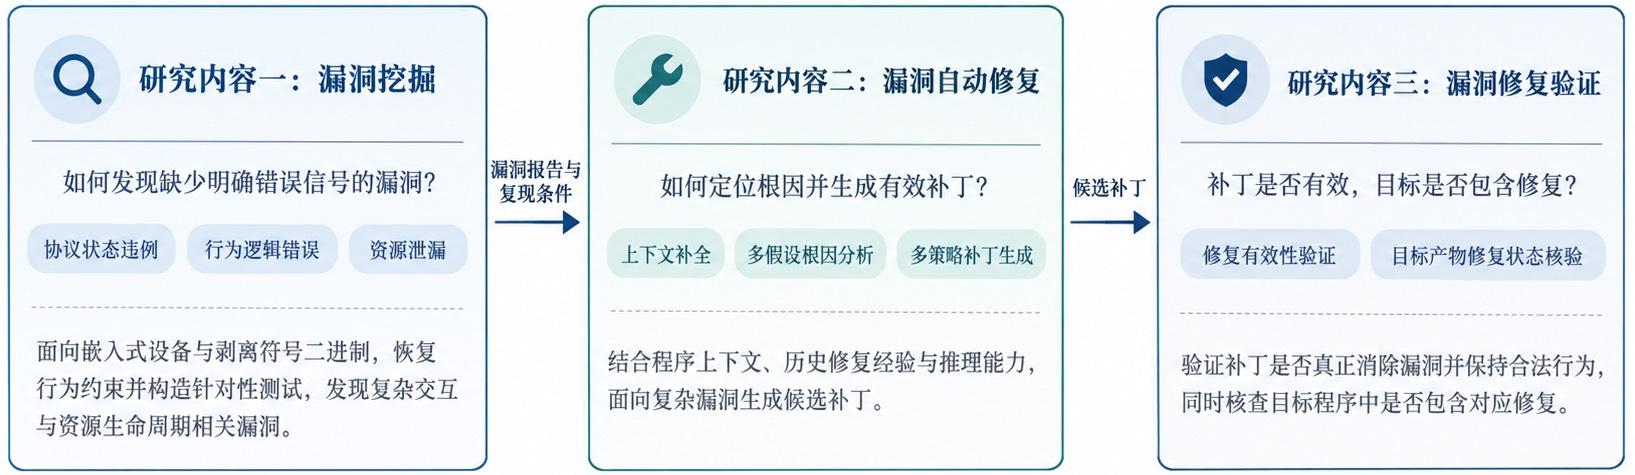
\includegraphics[width=\textwidth]{Img/overview.jpg}
\caption{研究内容总览}
\label{fig:overview}
\end{figure}

\subsection{研究目标}
\label{sec:research-objectives}

漏洞治理不仅需要发现潜在的安全缺陷，还需要针对漏洞形成有效修复，并确认修复满足相应安全要求、进入实际部署程序。仅发现漏洞或生成补丁，尚不足以确认目标系统中的相应风险已经消除。因此，本课题围绕“发现问题—生成修复—确认修复”的研究主线，探索大模型语义理解、智能体推理与程序分析相结合的方法，提升漏洞治理关键环节的自动化水平与结果可靠性。总体研究框架如图~\ref{fig:framework}~所示。

在漏洞挖掘环节，本课题重点关注嵌入式设备与剥离符号二进制场景中的协议状态违例、行为逻辑错误和资源泄漏等问题。此类问题的发现不仅需要触达相关执行路径，还需要判断程序行为是否违反协议、接口或资源生命周期要求。为此，拟研究受限信息条件下的行为约束恢复与针对性测试方法，将复杂交互中的状态变化与安全要求联系起来，提高对不易通过崩溃信号直接识别的漏洞的发现能力。

在漏洞修复环节，漏洞报告所指向的异常位置未必是实际需要修改的根因位置，而上下文缺失与过早收敛于单一解释，也可能限制修复策略的选择% TODO: 补充文献 hero（上下文缺失/过早收敛单一解释）。因此，本课题拟研究上下文增强与证据驱动的根因分析方法，结合历史修复经验开展多假设推理与多策略补丁生成，增强从漏洞表现追溯根因、从根因形成有效修改的能力，提高复杂漏洞自动修复的准确性与有效性。

在漏洞修复验证环节，补丁通过已知漏洞触发测试与功能测试，并不能充分说明漏洞根因已经消除\cite{rrbench}；同时，参考补丁的存在也不能直接证明实际部署的二进制包含对应修复\cite{zhang2026agenticppt}。为此，本课题拟从修复有效性与目标产物修复状态两个层面开展研究：一方面检查补丁是否满足漏洞相关安全要求并保持必要的合法行为，另一方面分析目标程序是否包含对应修复，提高对不完整修复、功能回归及修复缺失的识别能力。

基于上述目标，本课题形成\textbf{基于智能体的漏洞挖掘、基于智能体的漏洞自动修复、基于智能体的漏洞修复验证}三个研究内容。三者分别面向漏洞发现、候选补丁生成与修复结果确认，在任务目标上逐步衔接，共同为从漏洞识别到修复确认提供方法与技术支撑。

\begin{figure}[htbp]
\centering
\begin{tikzpicture}[node distance=0.5cm]
  % ---- 应用层 ----
  \node[smallbox, text width=2.9cm] (c1) {\textbf{内容一}\\漏洞挖掘};
  \node[smallbox, text width=2.9cm, right=1.1cm of c1] (c2) {\textbf{内容二}\\漏洞自动修复};
  \node[smallbox, text width=2.9cm, right=1.1cm of c2] (c3) {\textbf{内容三}\\漏洞修复验证};
  \draw[arr] (c1) -- node[above, font=\scriptsize]{PoC/根因} (c2);
  \draw[arr] (c2) -- node[above, font=\scriptsize]{候选补丁} (c3);
  \draw[darr] (c3.south) .. controls +(0,-0.55) and +(0,-0.55) .. node[below, font=\scriptsize]{安全规约反哺} (c1.south);
  \begin{scope}[on background layer]
    \node[layerbox, fit=(c1)(c2)(c3), label={[layerlabel]north west:应用层：漏洞攻防闭环}] (applayer) {};
  \end{scope}
  % ---- 方法层 ----
  \node[module, below=0.9cm of applayer, align=center] (method) {%
    \textbf{方法层：统一语义建模与智能体推理增强}\\
    漏洞语义表示 \quad 补丁语义表示 \quad 修复语义表示 \quad 跨环节能力迁移};
  % ---- 基础设施层 ----
  \node[module, below=0.4cm of method, align=center] (infra) {%
    \textbf{智能体基础设施层：Agent Harness 与工具链}\\
    规划—执行—反思循环 \quad 工具调用接口 \quad 上下文与记忆管理\\
    二进制分析（binutils/Ghidra）\quad 源码分析 \quad 模糊测试 \quad 符号执行};
  % ---- 数据层 ----
  \node[module, below=0.4cm of infra, align=center] (data) {%
    \textbf{数据与基准层：评估基础设施}\\
    语义漏洞基准（拟建）\quad RRBench~\cite{rrbench} \quad 561-CVE PPT 基准（已建）\cite{zhang2026pptempirical}};
\end{tikzpicture}
\caption{总体研究框架}
\label{fig:framework}
\end{figure}


\subsection{研究内容一：基于智能体的漏洞挖掘方法}

\textbf{主要研究内容}：语义/逻辑漏洞（如认证绕过、状态机错误、配置驱动缺陷）不产生崩溃信号，长期缺乏高效的自动化挖掘手段，是 IoT 与嵌入式固件安全中的突出短板。其核心难点在于：此类漏洞的触发路径通常由内部状态、配置、时序与外设响应等\textbf{自因变量}共同决定，传统输入驱动的模糊测试难以在错误的维度上有效探索；同时，语义漏洞的判定依赖人工构造的策略与规约，oracle 的缺失使自动化检测难以规模化。本研究内容旨在通过统一建模自因变量、自动构造语义 oracle、设计自因变量感知的智能体模糊测试，突破漏洞挖掘的自动化瓶颈，扩展可检测漏洞的类型与规模。

当前工作存在\textbf{自因变量难以统一建模、语义 oracle 难以自动构造}的挑战，因此，本文提出\textbf{自因变量感知的多智能体漏洞挖掘框架}。具体而言，首先综合静态分析与智能体推理，在固件二进制上识别各类自因变量，并统一表示为标注来源类型、取值空间与影响路径的自因变量格，使其成为模糊测试的一等探索维度；其次，利用智能体从协议 RFC、芯片数据手册与配置说明等自然语言文档中自动提取安全不变式，并编译为可执行的运行时监测点与断言，解决 oracle 自动构造难题；最后，设计规划—执行—验证三智能体协同的模糊测试架构，由规划智能体根据覆盖率与不变式反馈规划探索策略，执行智能体在生成输入的同时主动翻转目标自因变量（如注入中断、修改 NVRAM、模拟外设响应），验证智能体检查不变式违背并报告候选漏洞，并配套 PoC 生成与根因定位能力。

\textbf{预期目标}：构建基于智能体的漏洞挖掘系统，在真实 IoT 固件与合成基准上验证有效性，相比现有最优模糊测试方法在漏洞发现数量上提升 $\geq$ 5 倍，自因变量覆盖率 $\geq$ 70\%，安全 oracle 自动构造准确率 $\geq$ 80\%，在认证绕过、状态机错误与配置驱动缺陷三类典型漏洞上各发现若干真实漏洞并获得 CVE 编号，形成可复用的固件语义漏洞基准与工具原型。

\subsection{研究内容二：基于智能体的漏洞自动修复方法}

\textbf{主要研究内容}：漏洞自动修复是连接漏洞发现与漏洞消除的关键环节，其目标是自动定位漏洞根因、合成补丁并验证正确性。以 RRBench 为代表的大规模评估揭示了一个关键问题：现有智能体生成的"公开合理"补丁中，有相当比例（23.4\%）在私有安全性质检查下失败，且存在多个案例无法被任何系统正确修复~\cite{rrbench}。其根本原因在于：修复环节缺乏对"修复意图"的语义判定能力，智能体容易生成仅抑制特定 PoC、却未消除漏洞根因的过拟合补丁。值得注意的是，这一问题与补丁存在性测试中的"补丁语义判定"在本质上是对偶的——前者回答"生成的补丁是否构成有效修复"，后者回答"目标二进制是否包含修复"——两者均需对漏洞语义与修复语义进行深层建模。本研究内容旨在构建规约引导的可信自动修复框架，生成高质量候选补丁，并与研究内容三的修复验证方法形成"生成—验证"协同。

当前工作存在\textbf{部分规约下修复正确性难以验证、过拟合与回归难以系统抑制}的挑战，因此，本文提出\textbf{规约引导的智能体漏洞修复框架}。具体而言，首先依托统一的漏洞语义五元组表示（与研究内容一、三共享），将漏洞报告与 PoC 转化为结构化的根因语义表示；其次，借鉴 RRBench 私有 Oracle 的设计思想但将其自动化，利用智能体基于漏洞语义与代码上下文自动提取补丁必须满足的安全性质集合，既指导补丁生成又作为最终验证依据；再次，修复智能体在根因语义与安全规约的双重引导下进行多轮补丁生成与迭代，通过编译、公开测试与静态检查反馈持续修正候选补丁；最后，候选补丁交由研究内容三的修复验证环节进行 PPT 式的修复正确性判定，二者构成"生成—验证"对偶闭环，系统性抑制过拟合补丁与合法功能回归，实现部分规约下可信的自动修复。

\textbf{预期目标}：构建基于智能体的漏洞自动修复系统，在 RRBench 基准上将正确修复率从当前最优 69.6\% 提升至 $\geq$ 80\%，私有验证拒绝率降低 $\geq$ 50\%，在现有任何系统均无法正确修复的 14 个案例上成功修复 $\geq$ 4 个，形成可复用的安全规约自动提取工具链，并将方法论扩展至 C/C++ 等其他语言生态的修复基准。

\subsection{研究内容三：基于智能体的漏洞修复验证方法}

\textbf{主要研究内容}：补丁存在性测试（Patch Presence Testing，PPT）是连接漏洞披露与实际防护的关键环节，在软件供应链安全审计中具有不可替代的作用；同时，修复验证也是漏洞自动修复闭环的收官环节——自动合成的补丁是否真正消除漏洞根因，最终需要同样的补丁语义判定能力来回答。本人前期实证研究表明，前沿编码智能体已在端到端补丁存在性测试上达到与专用 SOTA 系统相当的性能~\cite{zhang2026agenticppt}，但其失败高度集中于两个环节：剥离二进制中的补丁定位，以及对后续版本中演化补丁的识别。前者源于源码级补丁意图与二进制级指令序列之间存在跨抽象层次的语义鸿沟，后者源于现有方法过度依赖补丁的形式特征而非修复意图。本研究内容旨在通过引入统一的漏洞语义表示，增强智能体在两个瓶颈环节上的推理能力，推动端到端修复状态验证从"可用"走向"可信、可扩展"，并将补丁语义判定能力对偶迁移至自动修复的补丁正确性验证。

当前工作存在\textbf{跨抽象层次补丁语义对齐困难、修复意图难以形式化}的挑战，因此，本文提出\textbf{语义先验引导的智能体修复验证增强框架}。具体而言，离线阶段利用智能体从 CVE 描述、补丁 diff 与源码上下文中提取"触发条件—危险操作—干预点—修复意图—上下文"的漏洞语义五元组，作为统一语义先验；在线阶段采用"粗—细"两阶段补丁定位，先用启发式规则快速缩小候选函数集，再以五元组为约束引导智能体在反汇编切片中进行置信度排序；针对演化补丁，提出基于修复意图的语义等价判定方法，不再追求形式上的补丁匹配，而是验证目标二进制中的干预是否实现了与原始补丁相同的安全语义。该框架在保持推理成本可控的前提下，系统性提升补丁定位准确率与演化补丁识别能力。

\textbf{预期目标}：构建基于智能体的端到端漏洞修复验证系统，在 561-CVE 基准上实现 DSR $\geq$ 0.98，在演化补丁子集上 DSR 提升 $\geq$ 15\%，在 Ubuntu 真实发行版包上保持 DSR $\geq$ 0.95，单例推理成本相比前沿配置增加不超过 10\%，形成可支撑大规模软件供应链审计与修复正确性判定的工具原型。

\subsection{预期目标与创新点}

（待撰写：分点列出理论创新、方法创新与系统/工具成果，以及预期论文与专利产出。）
%    三、课题主要研究内容、预期目标
\section{拟采用的研究方法、技术路线、实验方案及其可行性分析}

\subsection{基于智能体的漏洞挖掘方法}
\label{sec:discovery-method}

\subsubsection{问题定义与总体技术框架}
\label{sec:discovery-framework}

本研究面向嵌入式设备与剥离符号二进制，重点挖掘协议状态违例、跨调用行为逻辑错误和资源泄漏等不易通过崩溃信号识别的问题。针对行为约束不完整、内部状态难以观察以及错误判据不足等挑战，本文拟提出行为约束引导的状态探索与主动观测方法，将“如何触发潜在错误”与“如何观察并判断错误”联合考虑，通过针对性交互获得可复现的行为违例。

方法以目标设备或可执行二进制，以及能够获得的协议文档、接口说明、配置和正常交互样例为输入，不要求预先提供漏洞位置、触发程序或官方补丁。对于二进制可分析且具备运行时观察条件的目标，结合静态分析与动态观察辨识安全相关状态；对于仅能进行设备交互的目标，则利用响应、后续操作结果及可用诊断信息推断状态，不假设能够获取内部变量或代码覆盖。按照“行为约束构建—状态辨识与主动观测—交互生成与反馈优化—候选漏洞确认”的路线开展，技术路线如图~\ref{fig:mining-route}~所示，输出包含约束依据、触发条件、交互序列及安全影响的漏洞报告。

\begin{figure}[htbp]
\centering
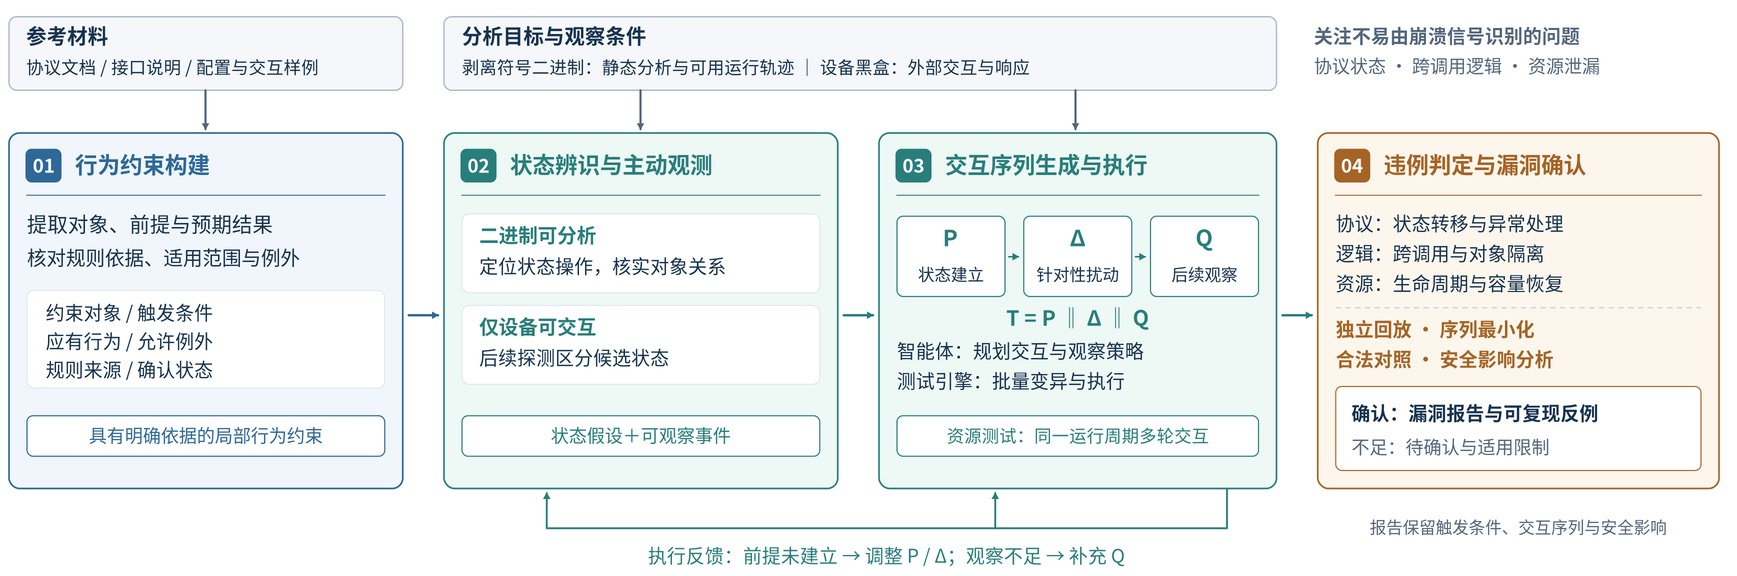
\includegraphics[width=\textwidth]{Img/漏洞挖掘.jpg}
\caption{基于智能体的漏洞挖掘技术路线}
\label{fig:mining-route}
\end{figure}

\subsubsection{行为约束引导的状态探索与主动观测}
\label{sec:discovery-technical-route}

首先，构建具有明确依据和适用范围的局部行为约束。利用大模型分析协议规范、接口说明及历史缺陷模式，提取约束对象、适用前提、触发事件和预期结果，再结合目标实现与交互信息检查其适用条件及事件映射。例如，资源约束不仅描述申请与释放操作，还需明确资源所属的会话、生命周期结束条件，以及允许延迟回收的例外。规则构建区分规范要求与实现观察，不将目标当前表现直接视为正确行为；缺少充分依据的规则保留为待验证假设。

其次，建立行为约束与目标可观察状态之间的对应关系。对于二进制目标，围绕约束涉及的操作定位状态建立、更新、使用和清理位置，并在具备条件时利用运行轨迹核实对象关系。对于黑盒设备，当即时响应不足以辨识状态时，由智能体构造具有区分能力的后续交互。例如，在规范要求注销后权限失效的场景中，除检查注销响应外，还需通过后续受保护操作观察原会话权限是否残留。系统根据结果更新候选状态假设；对可能改变被测状态的探测，通过相同前缀的独立回放进行对照，减少观察操作本身的干扰。

在此基础上，联合构造状态建立、条件扰动与后续观察序列，将一次测试表示为
\begin{equation}
    T = P \Vert \Delta \Vert Q,
    \label{eq:discovery-test-sequence}
\end{equation}
其中，$P$ 为建立目标状态的交互前缀，$\Delta$ 为针对特定约束的扰动，$Q$ 为用于辨识结果的观察后缀，$\Vert$ 表示序列连接。测试在保持无关语法和依赖条件的同时，改变消息顺序、取消时机或断连行为等目标条件，避免因前置步骤无效而始终停留在外围检查。对于资源累积问题，在同一运行周期中重复相关交互，再检查清理后的资源占用与后续申请能力。所有触发均限定在预设的交互能力和有效环境条件内，不以任意修改内部状态代替真实可达过程。

执行过程中，智能体负责约束解释、交互规划和观察策略调整，测试引擎负责批量变异、执行与结果采集。反馈除可获得的代码覆盖外，还包括约束前提是否成立、目标事件是否发生、状态假设是否得到区分以及资源回收条件是否满足。当前提未建立时补充交互前缀，扰动未触及目标行为时调整测试条件，结果无法判定时增加观察后缀，从而将测试预算用于具体的触发或观察缺口。

最后，根据约束类型构造相应判据：协议类检查状态转移及异常消息处理是否符合要求，跨调用逻辑类检查取消、回滚和对象隔离等行为关系，资源类检查生命周期结束后的资源残留与容量恢复。判定针对目标的实际行为，而不是将测试输入不合法直接视为漏洞。资源增长或等待超时仅作为候选信号，需要结合明确的回收条件与正常路径对照排除合法缓存和延迟清理。对候选问题进行独立回放、序列最小化和安全影响分析，排查规约误解与环境偏差；观察不足时保留不确定结论，不以模型判断替代可验证证据。

\subsubsection{实验方案与可行性分析}
\label{sec:discovery-evaluation}

实验拟按照可控软件对象、剥离符号二进制和真实设备逐步开展。在可控对象上利用源码和完整执行信息建立评价依据，但按实验设置限制被测系统能够访问的信息；随后分别评价剥离二进制与设备黑盒条件下的发现能力。测试对象覆盖协议状态、跨调用行为及资源生命周期相关缺陷，已知漏洞回溯与未知漏洞发现分别报告，目标漏洞的官方补丁和事后测试不进入发现阶段。

对比方法包括适用的状态感知模糊测试、规则驱动测试，以及使用相同模型、工具权限和预算的通用智能体。通过移除行为约束、主动观测和反馈调度等模块，评价各项设计的贡献，并比较持续多轮测试与逐轮重置对资源问题发现的影响。主要指标包括独立确认的缺陷与安全漏洞数量、首次确认时间、误报比例、无法判定比例及完整分析成本；状态覆盖与有效交互比例用于解释方法效果，不替代最终漏洞判定。

实现上拟复用二进制分析、模糊测试和设备交互工具，将新增研究集中于行为约束映射、触发与观察序列的联合生成，以及分类判据的可靠执行。初期选择具备明确协议或接口说明、可重复运行的目标验证核心机制，再逐步扩展至信息和观察能力受限的设备。对于环境难以复现或约束无法确认的案例，记录相应限制并分开分析，以控制实施风险并明确方法适用范围。

\subsection{基于智能体的漏洞自动修复方法}
\label{sec:repair-method}

\subsubsection{问题定义与总体技术框架}
\label{sec:repair-framework}

本研究面向已报告漏洞的源码自动修复，重点解决漏洞表现位置与实际修复位置不一致、上下文信息不完整，以及模型根因推理过早收敛和补丁生成同质化等问题。本文拟采用分层上下文构建、检索增强的多假设根因分析与多策略补丁生成相结合的方法，逐步完成从漏洞相关位置到根因解释、再到候选修复的分析过程，减少对准确修复位置和固定补丁模式的依赖。

方法以项目源码、漏洞相关位置及对应的 漏洞 类别为输入。其中，漏洞相关位置可以是异常触发或表现位置，不要求预先指出应修改的语句或函数。整体按照“漏洞上下文构建—多假设根因分析—多策略补丁生成”的路线开展，通过不同分析角色完成源码裁剪、依赖补全、根因推理和候选生成，无需针对修复任务进行模型微调。系统输出细化后的修复区域、根因分析报告及候选补丁集合，补丁是否满足安全要求则由后续独立验证确认。

\subsubsection{上下文增强与多假设推理驱动的补丁生成}
\label{sec:repair-technical-route}

首先，采用分阶段分析构建漏洞相关上下文。以报告位置为起点，引导大模型沿前向和后向分析数据依赖与控制依赖，保留与漏洞传播、危险操作及其前置条件相关的代码，裁剪无关实现，形成初始切片。随后，由依赖分析角色检查缺失的变量定义、函数调用及隐式状态关联，结合指针别名、共享状态和操作副作用，从源码仓库中补充相关代码。最后，由安全分析角色检查现有上下文是否足以解释漏洞，对缺失的辅助函数、数据结构和领域逻辑继续检索，并重新判断实际需要修改的程序区域。该过程以降低噪声、覆盖根因和保留必要的定义--使用关系为目标，而不是将报告位置直接作为补丁插入位置。

其次，构建支持根因分析的历史漏洞知识库。以 ReposVul 中的真实漏洞修复案例为基础，保存 漏洞 类别、漏洞代码、根因描述和补丁差异，分别对代码与根因文本进行向量化，并按 漏洞 类别组织检索分区。针对当前漏洞，智能体先依据增强后的上下文生成初始根因解释，但仅将其作为检索线索，不直接作为最终结论。随后，在对应类别中分别使用漏洞代码和初始根因描述开展余弦相似度检索，得到代码相似性与根因相似性两个排序列表。

为结合不同检索信号，采用倒数排名融合（Reciprocal Rank Fusion，RRF）计算案例的综合相关性：
\begin{equation}
    \operatorname{RRF}(e)
    =
    \sum_{j \in \{\mathrm{code},\,\mathrm{rca}\}}
    \frac{1}{k + \operatorname{rank}_{j}(e)},
    \label{eq:repair-rrf}
\end{equation}
其中，$e$ 表示历史案例，$\operatorname{rank}_{j}(e)$ 表示其在代码或根因检索通道中的排名，$k$ 为平滑常数。该方法在排序层面融合信息，避免直接拼接较长代码与较短根因描述造成信息不均衡。选取融合排名靠前的案例，将其根因说明和补丁差异作为参考，引导智能体提出多种候选根因解释，再结合初始分析形成结构化根因报告。漏洞 类别用于限定检索范围，而不直接决定当前漏洞的根因或修复模板。

在根因报告形成后，利用更新后的解释再次检索修复案例。具体而言，重新编码最终根因报告，更新根因通道的案例排序，并与已有代码通道排序进行融合，获得更贴近当前漏洞机制的修复参考。与仅在分析开始时检索一次相比，这一步使补丁生成所使用的历史经验能够随根因理解的变化而调整，减少初始解释偏差对后续生成的持续影响。

最后，通过五种互补策略引导补丁生成。最小修复以低侵入性修改直接处理核心根因；稳健修复采用成熟的安全实现替换危险编码模式；架构修复通过设计层面的调整减少产生危险行为的可能；增强型最小修复在局部修改基础上补充稳健性检查；局部架构修复结合安全实现替换与局部设计改进，在修改范围和结构调整之间取得平衡。智能体结合漏洞上下文、根因报告与更新后的参考案例，分别生成不同策略下的候选补丁，使候选差异体现在实际修复方式，而不只是代码表述变化。

各候选补丁保留对应的根因解释和修改依据，形成供后续验证的修复集合。本阶段关注有效修复方案的生成与覆盖，不以模型对补丁的自我评价代替正确性验证，也不预设修改最少或最接近官方补丁的方案必然正确。

\subsubsection{实验方案与可行性分析}
\label{sec:repair-evaluation}

实验拟采用 APPATCH 中的真实漏洞案例评价整体修复能力，并利用 InterPVD 中触发位置与修复位置跨函数分离的案例，评价不准确定位条件下的上下文构建与根因重定位能力。历史知识库与测试集按漏洞实例去重，排除测试漏洞对应的修复案例，避免检索直接暴露目标补丁。系统可访问漏洞源码、报告位置和类别信息，参考补丁仅用于评价，不进入目标漏洞的生成过程。

对比方法包括直接提示生成、APPATCH，以及 VulRepair、VulMaster 等修复方法。其中，提示式方法在相同基础模型和候选生成预算下进行比较，训练式方法则按其模型配置独立报告。主要指标包括修复召回率、补丁准确率和 F1 值：修复召回率衡量至少获得一个正确候选的漏洞比例，补丁准确率衡量生成候选中正确补丁的比例；同时统计根因分析准确率、不同模型下的表现及单例时间和推理成本。

\subsection{基于智能体的漏洞修复验证方法}

\textbf{拟解决的关键问题}：智能体在端到端漏洞修复验证（以补丁存在性测试为核心任务）中的两大瓶颈——\textbf{剥离二进制中的补丁定位}与\textbf{演化补丁识别}。前期实证研究表明，前者占弱模型配置独有失败的 95.2\%，后者是鲁棒性测试的主要失分点~\cite{zhang2026agenticppt}。两者本质上都源于跨抽象层次补丁语义对齐困难、修复意图难以形式化：源码级补丁意图与二进制级指令序列之间存在语义鸿沟，且现有方法过度依赖补丁的形式特征而非修复意图。

\textbf{技术方案}：针对上述问题，本文提出\textbf{语义先验引导的智能体修复验证增强框架}，整体技术路线如图~\ref{fig:verify-route} 所示，包含三个核心模块：

\begin{figure}[htbp]
\centering
\begin{tikzpicture}[node distance=0.45cm]
  \node[module] (m1) {%
    \textbf{模块一：漏洞语义先验提取}（离线，一次/漏洞）\\
    CVE 描述 + 补丁 diff + 源码上下文 $\xrightarrow{\text{智能体推理}}$\\
    漏洞语义五元组 $\langle$触发条件, 危险操作, 干预点, 修复意图, 上下文$\rangle$};
  \node[module, below=of m1] (m2) {%
    \textbf{模块二：语义引导的补丁定位}（在线，核心创新）\\
    粗定位：字符串/常量/导入表启发式 $\rightarrow$ 候选函数集\\
    细定位：五元组约束 + 反汇编切片 $\rightarrow$ Top-K 补丁候选区\\
    置信度排序：基于语义匹配度的候选排序};
  \node[module, below=of m2] (m3) {%
    \textbf{模块三：演化补丁的语义等价判定}（在线，核心创新）\\
    干预点识别：定位补丁实际修改的二进制指令\\
    修复意图比对：判断干预是否实现"修复意图"（而非形式匹配）\\
    不变式检查：验证修复后是否满足语义不变式};
  \draw[arr] (m1) -- (m2);
  \draw[arr] (m2) -- (m3);
\end{tikzpicture}
\caption{基于智能体的漏洞修复验证技术路线}
\label{fig:verify-route}
\end{figure}

\begin{itemize}
  \item \textbf{模块一：漏洞语义先验提取}。离线阶段利用智能体从 CVE 描述、补丁 diff 与源码上下文中提取漏洞语义五元组，作为统一语义先验，替代现有方法仅依赖原始补丁 diff 的浅层表示。
  \item \textbf{模块二：语义引导的补丁定位}。在线阶段采用"粗—细"两阶段定位：先用传统启发式（字符串、常量、导入表）快速缩小候选函数集，再将五元组作为约束注入智能体推理，引导其在候选函数中进行语义切片与置信度排序，输出 Top-K 补丁候选区域。
  \item \textbf{模块三：演化补丁的语义等价判定}。针对同一漏洞可能存在多种实现形式的修复（重构、拆分、合并等），不再追求"形式上的补丁匹配"，而是让智能体判断目标二进制中的干预点是否\textbf{实现了与原始补丁相同的修复意图}，并通过语义不变式进行交叉验证。
\end{itemize}

\textbf{可行性分析}：（1）数据基础充分：已构建 561 CVE 高保真基准与 12 组智能体配置的运行日志~\cite{zhang2026pptempirical,zhang2026agenticppt}，包含大量补丁定位与演化补丁的成功/失败案例，可直接用于方法设计与消融验证；（2）技术路线有实证支撑：前期工作已证明"丰富补丁元数据提升 DSR"与"补丁定位是主要瓶颈"两个关键结论，本方案是这两个结论的直接延伸，技术风险低；（3）工具链成熟：智能体框架（Codex / MiniSWEAgent）、二进制分析工具（binutils / Ghidra）与评估基准均已就绪，可快速进入实验迭代。

\textbf{实验方案}：基准沿用前期 561-CVE Source-Built Benchmark + Patch Evolution Set + Ubuntu Packages Set；对比方法包括 Codex 原始配置、Lares~\cite{lares}、PPTSP~\cite{pptsp}、PS\textsuperscript{3}~\cite{ps3}、BinXray~\cite{binxray}；评估指标包括 DSR、Accuracy、补丁定位准确率、每例 token 成本与时延；消融实验分别验证三个模块的独立贡献。预期全配置 DSR $\geq$ 0.98，演化补丁子集 DSR 提升 $\geq$ 15\%，成本增加 $\leq$ 10\%；进一步将验证能力对偶迁移至修复场景，在 RRBench 生成补丁上验证修复正确性判定的有效性。%   四、拟采用的研究方法、技术路线、实验方案及其可行性分析
\section{已有科研基础与所需的科研条件}

\subsection{已有科研基础}

本人围绕软件安全、漏洞分析与智能体安全方向开展了较为系统的文献调研和研究积累，已阅读并跟踪漏洞挖掘、自动漏洞修复、补丁验证、大语言模型与智能体应用于软件安全等领域的大量国内外研究工作，对传统程序分析方法、基于大模型的智能分析方法以及智能体驱动的软件安全研究范式具有较好的知识基础。通过前期调研，掌握了漏洞治理过程中漏洞发现、自动修复和修复验证等关键环节的发展现状与主要技术挑战，为后续开展基于智能体的漏洞挖掘与修复研究奠定了理论基础。

在漏洞修复验证方向，已开展了较为深入的研究工作。针对补丁存在性测试领域长期缺乏系统性评估、现有方法在真实部署场景下能力边界不明确的问题，完成了《A Comprehensive Empirical Analysis of Patch Presence Testing: Capabilities, Limitations, and Paths Forward》研究工作，并已被 \textit{ISSTA 2026} 录取~\cite{zhang2026pptempirical}。该工作首次针对补丁存在性测试开展系统性实证分析，构建大规模、高质量评测数据集，对现有代表性方法进行统一评估，分析影响检测效果的关键因素及失败原因，为后续智能体方法在补丁验证领域的发展提供了重要参考。

在上述研究基础上，进一步探索了基于智能体的端到端补丁存在性测试方法，完成了《Understanding Coding Agents for Patch Presence Testing》研究工作，目前已投稿~\cite{zhang2026agenticppt}。该工作将研究对象从传统专用分析工具扩展到通用编码智能体，系统分析智能体在补丁存在性测试任务中的能力边界，并提出面向该任务的智能体框架设计。实验结果表明，基于智能体的方法能够在真实二进制分析场景中达到与现有专用工具相当的性能，同时揭示了补丁定位和补丁演化识别等关键挑战，为后续研究智能体驱动的软件安全分析提供了实践基础。

在漏洞自动修复方向，已参与构建面向真实 Rust 漏洞的仓库级智能体修复评测基准《RRBench: A Repository-Level Benchmark for Agentic Repair of Real-World Rust Vulnerabilities》，目前已投稿~\cite{rrbench}。该工作针对现有漏洞自动修复评测中仅依赖 PoC 和功能测试、难以判断补丁是否真正恢复漏洞安全性质的问题，构建了包含真实漏洞案例、公开修复任务和独立安全验证机制的评测基准。通过对现有通用智能体修复能力的系统评估，发现当前智能体虽然能够生成大量表面有效的补丁，但仍存在根因理解不足、安全性质恢复不完整等问题。该工作为进一步研究基于智能体的漏洞自动修复方法、提升补丁生成可靠性提供了数据基础和问题依据。

综上，本人已在漏洞修复验证和智能体驱动漏洞分析方向形成了一定研究积累。其中，补丁存在性测试相关工作建立了对修复状态验证问题的系统认识，智能体补丁验证工作探索了端到端智能体解决方案，而漏洞修复评测基准工作进一步揭示了当前自动修复方法面临的关键挑战。这些研究基础为本课题后续围绕漏洞挖掘、漏洞自动修复以及漏洞修复验证三个方向开展深入研究提供了支撑。

\subsection{所需科研条件}

本课题研究需要的软件环境主要包括漏洞分析工具、程序分析框架、二进制分析工具以及大语言模型智能体开发环境。在漏洞挖掘方向，需要使用静态分析、动态分析、模糊测试和二进制分析工具，支持嵌入式设备、固件及复杂软件系统中的漏洞发现研究；在漏洞自动修复和修复验证方向，需要构建基于大语言模型的智能体框架，并结合代码分析、编译测试和漏洞验证环境开展实验。

硬件方面，需要具备支持大规模程序分析、大语言模型调用以及智能体实验运行的计算资源，包括高性能 CPU、GPU 服务器以及存储环境。同时，需要收集和维护真实开源项目、漏洞数据库、固件样本以及软件供应链组件等实验数据，为方法验证和系统评估提供基础。

目前，课题组已具备开展相关研究所需的软件安全研究环境，包括漏洞分析工具链、服务器计算资源以及大规模软件项目分析环境。同时，本人前期已积累漏洞数据构建、二进制分析、智能体框架开发和实验评测经验，能够支撑本课题后续研究工作的开展。
% 五、已有科研基础与所需的科研条件
\section{研究工作计划与进度安排}

\begin{enumerate}
  \item \textbf{2026.09 -- 2027.03}：完成研究内容一。构建自因变量统一建模与语义 oracle 自动构造方法，实现多智能体语义漏洞挖掘原型，建设固件语义漏洞基准，撰写并发表研究内容一论文。
  \item \textbf{2027.03 -- 2027.12}：完成研究内容二。实现规约引导的智能体漏洞修复框架，在 RRBench 上完成系统评估，撰写并发表研究内容二论文。
  \item \textbf{2028.01 -- 2028.10}：完成研究内容三。设计并实现语义先验引导的智能体修复验证（PPT 增强）框架，在 561-CVE 基准上完成对比与消融实验，撰写并发表研究内容三论文。
  \item \textbf{2028.10 -- 2029.06}：完成三个研究内容的端到端闭环集成与验证，整理成果，撰写博士学位论文，准备答辩。
\end{enumerate}

（注：以上时间节点为初步规划，可按实际学制与导师意见调整。）
%   六、研究工作计划与进度安排
%---------------------------------------------------------------------------%
% 正文章节
%-
%-> 后置部分：参考文献
%-
\artxifstreq{\artxbib}{bibtex}{% 使用 bibtex
    \bibliography{Biblio/ref}%
}{%
    \printbibliography%
}
\end{document}
%---------------------------------------------------------------------------%
